\documentclass[english]{kththesis}

\usepackage[style=numeric,sorting=none,backend=biber]{biblatex}
\usepackage[acronym, section=section, nonumberlist, nomain, nopostdot]{glossaries}
\usepackage[perpage,symbol]{footmisc}
\usepackage[parfill]{parskip} % Linebreak paragraphs instead of indent

\usepackage{longtable}
\usepackage{booktabs}
\usepackage{enumitem}

\usepackage{xcolor}     % Remove after \todo has been removed
\usepackage{tabularx}   % For additional table formatting
\usepackage{subcaption} % For subfigure support
\usepackage{pgfmath}    % --math engine
\usepackage{array}      % For table wrapping
\usepackage{graphicx}   % Support for images
\usepackage{float}      % Support for more flexible floating box positioning
\usepackage{setspace}   % For fine-grained control over line spacing
\usepackage{listings}   % For source code listing
\usepackage{tabularx}   % For simple table stretching
\usepackage{multirow}   % Support for multirow colums in tables
\usepackage{url}        % Support for breaking URLs
\usepackage{hyperref}
\usepackage[all]{hypcap}  % prevents an issue related to hyperref and caption linking
%% setup hyperref to use the darkblue color on links
\hypersetup{colorlinks,breaklinks,
            linkcolor=darkblue,urlcolor=darkblue,
            anchorcolor=darkblue,citecolor=darkblue}

%% Some definitions of used colors
\hyphenpenalty=15000\tolerance=1000 % to reduce hyphenation
\definecolor{darkblue}{rgb}{0.0,0.0,0.3} %% define a color called darkblue
\definecolor{darkred}{rgb}{0.4,0.0,0.0}
\definecolor{red}{rgb}{0.7,0.0,0.0}
\definecolor{lightgrey}{rgb}{0.8,0.8,0.8} 
\definecolor{grey}{rgb}{0.6,0.6,0.6}
\definecolor{darkgrey}{rgb}{0.4,0.4,0.4}
\definecolor{aqua}{rgb}{0.0, 1.0, 1.0}

\usepackage[cache=false]{minted} %% For source code highlighting
\usemintedstyle{borland}

\usepackage{csquotes} % Recommended by biblatex

% set the chapter header
\renewcommand{\chaptermark}[1]{\markboth{#1}{}}

% to get rolling footnote numbers
\counterwithout{footnote}{chapter}

\newcolumntype{P}[1]{>{\endgraf\vspace*{-\baselineskip}}p{#1}}

% custom macros
\newcommand{\footnotelink}[2]{\footnote{\url{#1} | Accessed #2}}
\newcommand{\todo}[0]{\colorbox{orange}{TODO}}

% The list of acronyms and abbreviations should be in alphabetical order based on the spelling of the acronym or abbreviation.
\makeglossaries

\newacronym{IOT}{IoT}{Internet of Things}

\title{Hacking Into Someone's Home using Radio Waves}
\subtitle{Ethical Hacking of Securitas' Alarm System}
\alttitle{Hacka in i Någons Hem med hjälp av Radiovågor}
\altsubtitle{Etiskt Hackning av Securitas Hemlarmsystem}

\authorsLastname{Lindeberg}
\authorsFirstname{Axel}
\email{alindeb@kth.se}
\kthid{alindeb}
\authorsSchool{\schoolAcronym{EECS}}
\programcode{CDATE}

\supervisorAsLastname{Johnson}
\supervisorAsFirstname{Pontus}
\supervisorAsEmail{pontusj@kth.se}
\supervisorAsKTHID{pontusj}
\supervisorAsSchool{\schoolAcronym{EECS}}
\supervisorAsDepartment{Division of Network and Systems Engineering}

\examinersLastname{Lagerström}
\examinersFirstname{Robert}
\examinersEmail{robertl@kth.se}
\examinersKTHID{robertl}
\examinersSchool{\schoolAcronym{EECS}}
\examinersDepartment{Division of Network and Systems Engineering}

\hostorganization{Försvarsmakten (Swedish Armed Forces)}

\addbibresource{references.bib}

\begin{document}
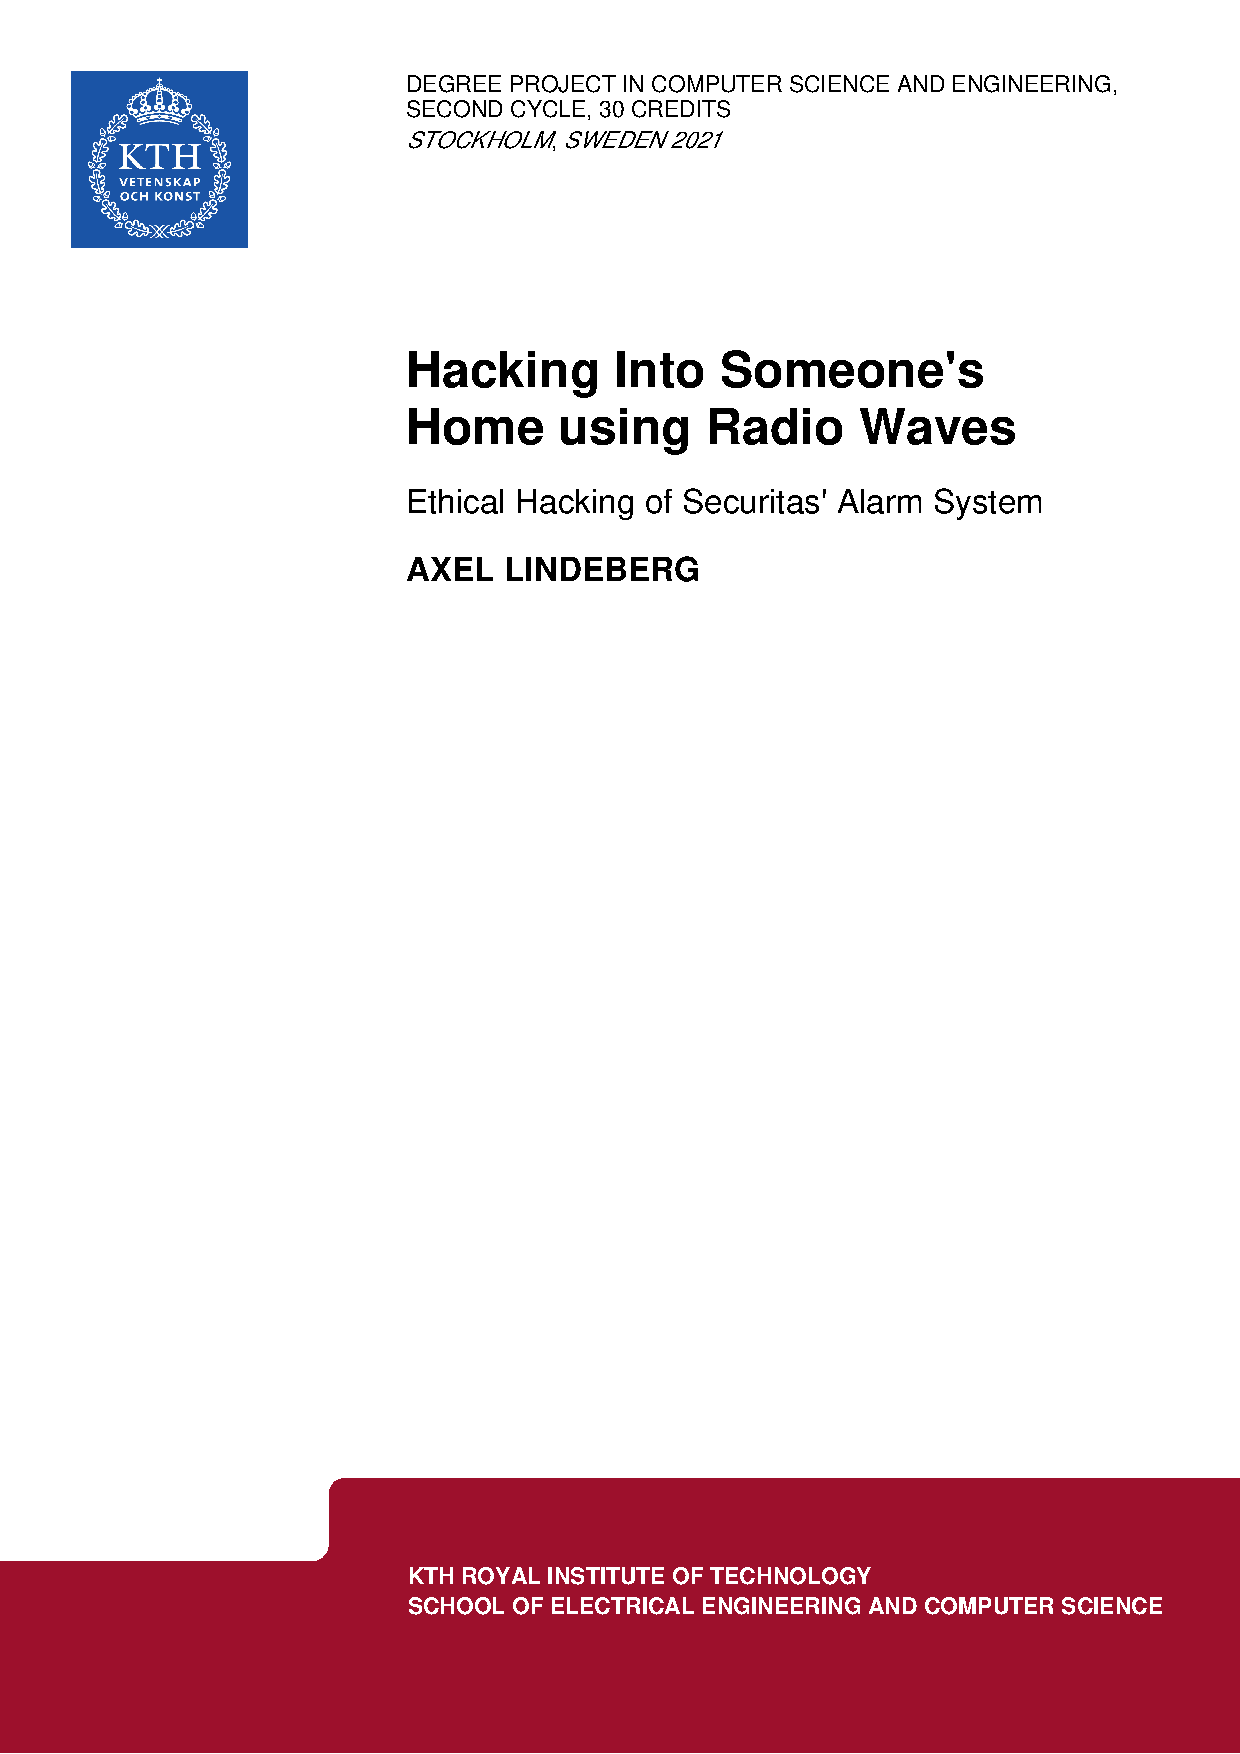
\includepdf[pages=1,pagecommand={\thispagestyle{empty}},width=\paperwidth]{kth-cover.pdf}
\thispagestyle{empty}\cleardoublepage

\titlepage
\bookinfopage

\frontmatter
\setcounter{page}{1}

% ---- English Abstract ----
\begin{abstract}
\markboth{\abstractname}{}
% Keep in mind that most of your potential readers are only going to read your title and abstract. This is why it is important that the abstract give them enough information that they can decide is this document relevant to them or not. Otherwise the likely default choice is to ignore the rest of your document.
% A abstract should stand on its own, i.e., no citations, cross references to the body of the document, acronyms must be spelled out, …
% Write this early and revise as necessary. This will help keep you focused on what you are trying to do.

% Write an abstract (250 and 350 words) with the following components:
%  - What is the topic area? (optional) Introduces the subject area for the project.
%  - Short problem statement
%  - Why was this problem worth a Master’s thesis project? (i.e., why is the problem both significant and of a suitable degree of difficulty for a Master’s thesis project? Why has no one else solved it yet?)
%  - How did you solve the problem? What was your method/insight?
%  - Results/Conclusions/Consequences/Impact: What are your key results/conclusions? What will others do based upon your results? What can be done now that you have finished - that could not be done before your thesis project was completed? The presentation of the results should be the main part of the abstract.
\todo

\subsection*{Keywords}
% Choosing good keywords can help others to locate your paper, thesis, dissertation, … and related work.}
% Choose the most specific keyword from those used in your domain, see for example:
% ACM's Computing Classification System (2012) or
% (2014) IEEE Taxonomy. 
% Mechanics:
% - The first letter of a keyword should be set with a capital letter and proper names should be capitalized as usual.
% - Spell out acronyms and abbreviations.
% - Avoid "stop words" - as they generally carry little or no information.
% - List your keywords separated by commas (",").
% Since you should have both English and Swedish keywords - you might think of ordering them in corresponding order (i.e., so that the nth word in each list correspond) - thus it would be easier to mechanically find matching keywords.
\todo

\end{abstract}

% ---- Swedish Abstract ----
\selectlanguage{swedish}
\begin{abstract}
% All theses at KTH are required to have an abstract in both English and Swedish.
% If you are writing your thesis in English, you can leave this until the final version. If you are writing your thesis in Swedish then this should be done first – and you should revise as necessary along the way.
% If you are writing your thesis in English, then this section can be a summary targeted at a more general reader. However, if you are writing your thesis in Swedish, then the reverse is true – your abstract should be for your target audience, while an English summary can be written targeted at a more general audience.
% The Swedish sammanfattning need not be a literal translation of the english abstract.
\todo

\subsection*{Nyckelord}
\todo

\end{abstract}

\clearpage

\selectlanguage{english}
\section*{Acknowledgments}
\markboth{Acknowledgments}{}
I would like to thank Fredrik Heiding, PhD student within cybersecurity at KTH, for helping me procure the alarm system investigated in this thesis, as well as the HackRF SDR, and navigating the KTH bureaucracy surrounding that process.

I would also like to acknowledge Professor Andreas Noack from the University of Applied Sciences Stralsund in Germany. Not only did he co-create the excellent tool \textit{Universal Radio Hacker} which was used extensively in this thesis. He also offered up a lot of his time in personally helping me when I initially felt way out of my depth with RF hacking by answering questions about the URH tool, RF communication in general, and figuring out how to capture good signals for this system.

Next, I would like to thank my girlfriend, Caroline, who had to hear me go on and on about radio waves and RF hacking for months, handle the stressful periods, for continuously proofreading the thesis, and for putting up with this whole situation during a pandemic. The same goes for the rest of my family.

I would, of course, like to thank my supervisor at Försvarsmakten. They gave me invaluable insights and expertise during this entire project. All the way from selecting what type of system to explore, to sharing their knowledge during the pentesting phase, to proofreading the final version. They also lent me more than enough of their time, meeting with me every week to discuss the thesis which I really appreciated.

Above all, I would like to thank my KTH supervisor Pontus Johnson. Before even starting this thesis, his excellent course Ethical Hacking (EN2720) opened my eyes to this entire field and was easily my favorite course at KTH. He also personally helped me get in contact with and recommended me to several organizations within the security industry during the search for a place to write my thesis as well as during my job hunt after graduation. During the thesis, Pontus also gave a lot of his time, answered questions, and gave excellent feedback and encouragement.

Lastly, a special thanks to KTH for these last five years!

\acknowlegmentssignature

% ---- Table of contents, etc ----
\fancypagestyle{plain}{}
\tableofcontents
\markboth{\contentsname}{}

\clearpage\listoffigures
\clearpage\listoftables
\clearpage\printglossary[type=\acronymtype, title={List of acronyms and abbreviations}]

\label{pg:lastPageofPreface}

\mainmatter
\chapter{Introduction} \label{ch:intro}
% Ofta kommer problemet och problemägaren från industrin där man önskar en specifik lösning på ett specifikt problem. Detta är ofta ”för smalt” definierat och ger ofta en ”för smal” lösning för att resultatet skall vara intressant ur ett mer allmänt ingenjörsperspektiv och med ”nya” erfarenheter som resultat. Fundera tillsammans med projektets intressenter (student, problemägare och akademi) hur man skulle kunna använda det aktuella problemet/förslaget för att undersöka någon ingenjörsaspekt och vars resultat kan ge ny eller kompletterande erfarenhet till ingenjörssamfundet och vetenskapen.
% 
% Examensarbetet handlar då om att ta fram denna nya ”erfarenhet” och på köpet löser man en del eller hela delen av det ursprungliga problemet.
% 
% Erfarenheten kommer ur en frågeställning som man i examensarbetet försöker besvara med tidigare och andras erfarenhet, egna eller modifierade metoder som ger ett resultat vilket kan användas för att diskutera ett svar på undersökningsfrågan.
% 
% Detta stycke skall alltså, förutom det ursprungliga ”smala” problemet, innehålla  vad som skall undersökas för att skapa ny ingenjörserfarenhet och/eller vetenskap.

% This chapter describes the specific problem that this thesis addresses, the context of the problem, the goals of this thesis project, and outlines the structure of the thesis.
% Give a general introduction to the area. (Remember to use appropriate references in this and all other sections)

Home automation and the number of connected devices in our home has exploded in recent years. The number of \gls{IOT} devices especially have increased dramatically. It is predicted there will be about 38 billion of them by 2025 \cite{ieee-iot}. Many of \gls{IOT} devices are connected to the internet and that fraction is bound to increase given the rise of 5G technology. While these devices can do amazing things, everything from smart speakers to connected refrigerators, they are hardly known for their security. While this is well known in the IT-security community, the general non-tech-savvy consumer are perhaps not as aware of the security considerations when bringing an \gls{IOT} device into their home.

A type of connected device that has become increasingly common and increasingly complex are smart Home Alarm Systems. They protect your house from intruders by sounding an alarm when an expected intrusion has occurred and often a security central is immediately notified and security personnel immediately sent to the site. These systems can be incredibly complex and can include multiple external peripherals like motion detectors, surveillance cameras, smoke detectors, smart locks, etc. In recent years their scope have expanded further and can now often control home automation systems like smart light bulbs, connected coffee machines, and even the lock to your door. Additionally, they can often be controlled remotely via mobile apps and web-portals. While these are undoubtedly useful features and undeniably provide protection against physical intrusion one might wonder how secure these systems are against cyberattacks and much of a focus the cybersecurity of these systems is to the companies behind them.

This thesis will examine the cybersecurity of a smart Home Alarm System from SecuritasHome. The SecuritasHome system is a Home Alarm System with features such as alarming the system using a remote keypad and a four-digit pin, smoke detection, motion-detection with a corresponding camera, and control of home automation devices. However, the main panel of the system (the \textit{brain of the system}) is connected to the internet, both the local network and the mobile 3G network. If one were to comprise the security of this system there could be devastating consequences, such as disarming the alarm and entering the house without setting it off.

\section{Research question} \label{ch:intro:research-question}
This report will try and answer the following research question:

\begin{quote}
    \textit{Is the SecuritasHome Home Alarm System secure against cyberattacks?}
\end{quote}

\noindent In particular, this question can be broken down into two parts:

\begin{itemize}
    \item What vulnerabilities are present in the system?
    \item How can the vulnerabilities be exploited?
\end{itemize}

\noindent The security analysis presented in this thesis was performed on the following firmware version: \texttt{HPGW-G 0.0.2.23F BG\_U-ITR-F1-BD\_BL.A30.20181117}. This was the latest version at the time, which was the spring of 2021.

\section{Background} \label{ch:intro:background}
% Present the background for the area. Set the context for your project – so that your reader can understand both your project and this thesis. (Give detailed background information in Chapter 2 - together with related work.)
% Sometimes it is useful to insert a system diagram here so that the reader knows what are the different elements and their relationship to each other. This also introduces the names/terms/… that you are going to use throughout your thesis (be consistent). This figure will also help you later delimit what you are going to do and what others have done or will do.
[TODO]

\section{Objectives} \label{ch:intro:objectives}
% State the purpose  of your thesis and the purpose of your degree project. Describe who benefits and how they benefit if you achieve your goals. Include anticipated ethical, sustainability, social issues, etc. related to your project. (Return to these in your reflections in Section~\ref{sec:reflections}.)

% Skilj på syfte och mål! Syfte är att förändra något till det bättre. I examensarbetet finns ofta två aspekter på detta. Dels vill problemägaren (företaget) få sitt problem löst till det bättre men akademin och ingenjörssamfundet vill också få nya erfarenheter och vetskap. Beskriv ett syfte som tillfredställer båda dessa aspekter.
% Det finns även ett syfte till som kan vara värt att beakta och det är att du som student skall ta examen och att du måste bevisa, i ditt examensarbete, att du uppfyller examensmålen. Dessa mål sammanfaller med kursmålen för examensarbetskursen. 
The objective of this thesis is to asses the security of the SecuritasHome Home Alarm System. In essence, the objective in terms of the degree project is to asses whether or not the system can be considered secure from an computer-security perspective. To achieve this a comprehensive security audit was made to the system, to investigate which attack vectors the system is vulnerable to. Considering the large attack surface of the system in question, given it's complexity and variety of features, some areas where delimited. More on this in \ref{ch:intro:delimitations}.

From the perspective of the host organization, \textit{Försvarsmakten}, the objectives were to asses the security of home alarm systems in general, which have become increasingly common. While these systems are generally considered effective against physical intrusion, less is sure about their security when it comes to cyberattacks. The host organization wanted a thorough investigation into the IT-security of such a system.

\section{Methodology} \label{ch:intro:methodology}
% Här anger du vilken vilken övergripande undersökningsstrategi eller metod du skall använda för att försöka besvara den akademiska frågeställning och samtidigt lösa det e v ursprungliga problemet. Ofta kan man använda ”lösandet av ursprungsproblemet” som en fallstudie kring en akademisk frågeställning. Du undersöker någon intressant fråga i ”skarpt” läge och samlar resultat och erfarenhet ur detta.\\
% Tänk på att företaget ibland måste stå tillbaka i sin önskan och förväntan på projektets resultat till förmån för ny eller kompletterande ingenjörserfarenhet och vetenskap (ditt examensarbete). Det är du som student som bestämmer och löser fördelningen mellan dessa två intressen men se till att alla är informerade.

% Introduce your choice of methodology/methodologies and method/methods – and the reason why you chose them. Contrast them with and explain why you did not choose other methodologies or methods. (The details of the actual methodology and method you have chosen will be given in Chapter~\ref{ch:methods}. Note that in Chapter~\ref{ch:methods}, the focus could be research strategies, data collection, data analysis, and quality assurance.) In this section you should present your philosophical assumption(s), research method(s), and research approach(es).
[TODO]

\section{Delimitations} \label{ch:intro:delimitations}
% Describe the boundary/limits of your thesis project and what you are explicitly not going to do. This will help you bound your efforts – as you have clearly defined what is out of the scope of this thesis project. Explain the delimitations. These are all the things that could affect the study if they were examined and included in the degree project.
The system under consideration of this thesis is very complex. It consists many features, applications, and physical peripherals. As such, there is unfortunately not enough time within the scope of a degree project to exhaustively consider the full attack surface. Some things were also delimited due to legal reasons. As such the following major delimitations were done early in the project:

\begin{itemize}
    \item The external cloud servers, hosted by \textit{Alarm.com}. Legally, the security of these could not be assesed.
    \item The 3G wireless telecommunication. This was primarily due to the custom hardware required and the well-known security of this encrypted protocol.
    \item The security of additional peripherals not included in the starter-kit, see \ref{ch:system:hardware}.
    \item The iOS mobile application. This was delimited for two primary reasons, the major one being time and the other being the author not having easy access to an iOS device.
    \item The Android mobile application. [Note: Maybe?]
\end{itemize}

\noindent Additionally, more fine-grained delimitations were done during the exploratory phase of the project. More on this in [REF].

\section{Structure of the thesis} \label{ch:intro:structure}
This report is structured in to the following chapters:
\begin{itemize}
    \item Chapter \ref{ch:intro} gives an introduction into the thesis and research question, as well as a brief introduction into the background of the subject area.
    \item TODO...
\end{itemize}

\chapter{Method} \label{ch:method}
The following chapter described the method used in this report. It is based on a seven step process to penetration testing by \textcite{weidman2014}. In the first part, this method is described. That is followed by how each of these seven steps were carried out on this thesis. Additionally, for the threat modeling phase a method outlined by \textcite{guzman2017iot} was used. This threat modeling process is described below.

\section{Penetration Testing methodology} 
In their book \citetitle{weidman2014}, \citeauthor{weidman2014} details a seven step process for penetration testing \cite{weidman2014}. This section firstly gives a brief description of all seven steps, and lastly outlines how each step was performed in this thesis.

Included in \citeauthor{weidman2014}'s method for penetration testing are the following seven steps:
\begin{enumerate}
    \item \textit{Pre-engagement}. This step involves communicating with the party that ordered the penetration test to be done. The goal of this step is to make sure both parties are on the same page and understanding of how the tests will be done. Things to agree upon, according to \citeauthor{weidman2014}, are scope, testing window, and clear authorization from the other party that you are legally allowed to assess the security of their system.
    \item \textit{Information Gathering}. This step includes what is known as \gls{OSINT}. \gls{OSINT} is the process of using publicly available sources of information to gather information about the system in question. These include search engines like Google, news articles, public government data, academic papers, etc \cite{steele2007open}. One might also use port scanners like \textit{Nmap}\footnotelink{https://nmap.org/}{2021-03-29} and other application scanners to gather information about the system. Additionally, one might listed in on the network traffic of the system to gain an understanding of it's behavior, using tools like \textit{WireShark}\footnotelink{https://www.wireshark.org/}{2021-04-01} for example.
    \item \textit{Threat Modeling}. This step involves mapping out the components of the system, based on the information from the previous step. From that, you think of potential attacks and vulnerabilities of the system, their potential impact, and likelihood of success. There are many different threat modeling techniques. More on this and the technique used in this report can be found in section \ref{ch:method:threat-modeling}.
    \item \textit{Vulnerability Analysis}. This step involves actively pentesting the system to discover vulnerabilities. This can be done for example through manually probing the system or by using vulnerability scanners like \textit{Metasploit}\footnotelink{https://www.metasploit.com/}{2021-03-29}, \textit{Burp Suite}\footnotelink{https://portswigger.net/burp}{2021-03-29}, or \textit{Nessus}\footnotelink{https://www.tenable.com/products/nessus}{2021-03-29}.
    \item \textit{Exploitation}. This step involves exploiting the vulnerabilities discovered in the previous step. By exploiting these, the goal is to perform some malicious act on the system, see \ref{ch:method:stride}.
    \item \textit{Post Exploitation}. After a successful exploit, this step involves analyzing the consequences of it. If the exploit involves access to a machine one might investigate the file system, look for possibilities of privilege escalation, etc. One asks how sever this successful exploit is to the overall security of the system.
    \item \textit{Reporting}. This final step involves summarizing the findings to the interested party. Crucially, if the findings are to be publicized one should adhere to the principle of responsible disclosure.
\end{enumerate}
What follows is a description of how each step above was applied in this thesis.

\subsection{Pre-engagement}
According to \citeauthor{weidman2014}'s method, the pre-engagement step is done in collaboration with the client. In this project, however, there is no clear client except the author and perhaps KTH and Försvarsmakten. The scope and expectations were continuously discussed during the course of the project. The companies behind the system (see \ref{fig:company-structure}) were not informed of the security analysis until after the project was finalized. Securitas, the seller of the system was contacted multiple times over phone via their customer support to verify the legality of security testing the system.

\subsection{Information Gathering}
The information gathering phase was done in several steps, the first one being \gls{OSINT}. Initially, the model number of all devices were gathered from either physical labels on the peripherals or from Securitas' website\footnotelink{https://www.securitashome.se/}{2021-03-29}. Using the search engine Google, the devices and their manufacturer \textit{Climax Technology} were quickly identified. From their website much more information about the system could be found, such as how the peripherals communicate and their proprietary \gls{RF} protocol\footnotelink{https://www.climax.com.tw/new/f1-features-new.php}{2021-03-29}. An additional resource was finding each component's FCC ID\footnotelink{https://www.fcc.gov/oet/ea/fccid}{2021-03-30}, from which one can find user manuals submitted to the FCC agency, official testing documentation, and more via \textit{fccid.io}, see chapter \ref{ch:system}.

\subsection{Threat Modeling}
Threat modeling involves building a thorough picture of the system and identifying all possible threats to the system. There are many different threat modeling techniques. The threat modeling technique used in this thesis is one outlined in the book \citetitle{guzman2017iot}. In their book, authors \citeauthor{guzman2017iot}, describe a threat modeling technique for IoT devices \citeauthor{guzman2017iot}, which features a 6 step process. More on this in section \ref{ch:method:threat-modeling}.

\subsection{Vulnerability Analysis}
[TODO]

\subsection{Exploitation}
[TODO]

\subsection{Post Exploitation}
[TODO]

\subsubsection{Reporting}
[TODO]

\section{Threat modeling for IoT devices} \label{ch:method:threat-modeling}
In their book \citetitle{guzman2017iot}, authors \citeauthor{guzman2017iot}, outline a six step process for threat modeling IoT devices. This is the threat modeling technique used in this thesis, the result of which can be found in section \ref{ch:threat-model}. The six steps of the process listed and described below:
\begin{enumerate}
    \item \textit{Identify IoT assets}. This initial step involves identifying all assets of the system you have an interest in protecting. Essentially, this list should include anything that could be a target or something negatively effected by an attack. This aids in identifying what an attacker might focus on when crafting an attack or pentesting the system. Can be presented as a simple table describing each asset.
    \item \textit{Create an IoT Device Architecture Overview}. Once all assets have been identified, the next step involves creating an architecture diagram. In their method, \citeauthor{guzman2017iot} include three components of this architecture breakdown. First is a list of all use cases of the system. This details what a regular user can do with the system and the steps of each. Second is a diagram of all components of the system, and how they communicate (what protocol for example). Components can include everything from external cloud servers, network equipment, and individual processes. This is usually presented visually, in a diagram depicting the system. Lastly, a list of all identified technologies used in the system is included. This list should include everything from operating systems, network protocols, and known applications. Any additional information about each, such as version number for example, should be included if known.
    \item \textit{Decompose the IoT Device}. This step includes analyzing application and protocol data flow of the system. Using this, one aims to locate vulnerable entry points of the system, either into physical devices or client applications. Additionally, entry points of higher privilege access should be noted and every single entry point of the system identified. An entry point could for example be a hosted web server on an IoT device or an open TCP port, the firmware of the device, or a mobile application.
    \item \textit{Identify Threats}. In this phase the threats to the system are identified. The documented data flows aid you in identifying potential threats. One can use a model of threats like STRIDE\cite{stride} to identify threats of different characteristics, see section \ref{ch:method:stride}. In their method, \citeauthor{guzman2017iot} propose adding two categories to the STRIDE model for IoT specific threats. The first one is \textit{Physical Security Bypass}, which involve vulnerabilities caused by the attacker having physical access to the device for some limited period of time. The second category is \textit{Supply Chain Issues}, which includes threats to the various technologies that the system relies on. This could be documented vulnerabilities in the hardware platform for example.
    \item \textit{Document Threats}. A few of the identified threat use cases will be documented in this step. For each, the target of the threat, the attack technique, and the potential countermeasures should be noted.
    \item \textit{Rate the Threats}. For each documented threat, one rates it's severity. The authors propose using a system like DREAD to give a score to each threat, based on a few different criteria like damage potential and reproducibility.
\end{enumerate}

\section{The STRIDE model} \label{ch:method:stride}
STRIDE is a model of threats used to identify threats to the cybersecurity of an IT system \cite{stride}. It was initially developed by Praerit Garg and Loren Kohnfelder at Microsoft as part of their threat modeling technique. It is a widely used mnemonic in the security industry to aid in recognizing threats\footnotelink{https://docs.microsoft.com/en-us/azure/security/develop/threat-modeling-tool-threats}{2021-03-29}. The following are the six properties that make up the acronym and a description of each:
\begin{itemize}
    \item \textbf{S}poofing identity. This means impersonating the identity of another user or component of the system. One example is obtaining a users login credentials and posing as that user.
    \item \textbf{T}ampering with data. This means modifying data in the system in a malicious manner that you were perhaps not meant to modify. An example is unauthorized modifications to data stored in a database.
    \item \textbf{R}epudiation. This means being able to claim you did not perform a certain action. An example would be to somehow be able to claim a transaction did not go through, thereby illegally receiving additional payment.
    \item \textbf{I}nformation disclosure. This means exposing information or data to users who are not meant to have access to it. An example is a database leak.
    \item \textbf{D}enial of service. This means denying access to a service. An example is making a web server unavailable to users by hitting it with heavy traffic, perhaps via a distributed \gls{DOS} attack.
    \item \textbf{E}levation of privilege. This means an unprivileged user gaining privileged access to the system, allowing them access to features of the system they were not meant to. An example is exploiting a vulnerability in a program or kernel to get access as a more privileged user on the machine (like root).
\end{itemize}

\chapter{System Under Consideration} \label{ch:system}
The following chapter gives a thorough explanation of the system under consideration of this thesis. The system in question is the \textit{SecuritasHome startpaket}, which is a home alarm system from Securitas. This starter-kit includes multiple hardware components, as well as access to software portals and mobile applications to control the system.

\section{The companies behind the system}
This section covers the structure of the three major companies behind the SecuritasHome Home Alarm System.

While the system is sold and branded by SecuritasHome, they actually have little to do with the actual hardware and software components of the platform, see figure \ref{fig:company-structure}. The hardware, related firmware, and proprietary radio wave protocol for communication between the components are manufactured and produced by a Taiwanese company called \textit{Climax Technology}\footnotelink{https://www.climax.com.tw/}{2021-04-01}. They are a major manufacturer of wireless home security systems and produce hardware for home consumer security. They design everything from smart home alarm systems, and smart garage door openers, to smart medical accessories for seniors. The software, like the web portal and mobile applications as well as some additional firmware, are developed by an American company called \textit{Alarm.com}\footnotelink{https://alarm.com/}{2021-04-01}. They are strictly a B2B (business to business) company, meaning they do not sell or advertise their product directly to the end consumer. Instead they outsource the sale and advertisement of the system to partner companies, one of them being Securitas. SecuritasHome merely sell, advertise, and put their brand on the product. Their main contribution to the system is in terms of real-time response to an alarm, connection to an alarm-central, and sending security personnel to respond to an active alarm breach. Consequently, when considering the cybersecurity of the system, Securitas is not strictly relevant. The two relevant parties are \textit{Alarm.com} and, considering the focus of this thesis, especially \textit{Climax Technology}.
\begin{figure}[!ht]
    \centering
    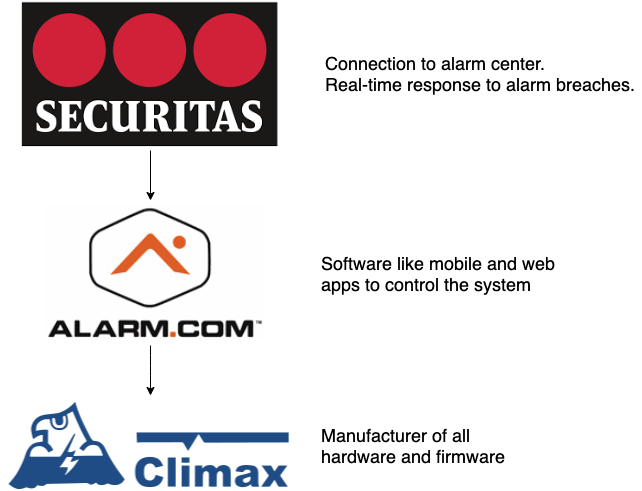
\includegraphics[width=0.7\textwidth]{images/company-structure.png}
    \caption{The companies behind the system.}
    \label{fig:company-structure}
\end{figure}

\section{Components and Software} \label{ch:system:components}
This section describes all the components and software of the system. Initially, all hardware components are described and their functionality. Lastly, all software components of the system are described. Note that the system supports many additional hardware components. The ones outlined below are only the ones part of the starter-kit.

\subsection{Hardware components} \label{ch:system:hardware}
The SecuritasHome starter-kit contains five hardware components, see figure \ref{fig:hardware-components}. These are described below. Note that the system supports many additional components, like smart locks for example. However, only the components included in the starter-kit are covered in this thesis.
\begin{figure}[!ht]
    \centering
    \begin{subfigure}[t]{0.33\textwidth}
        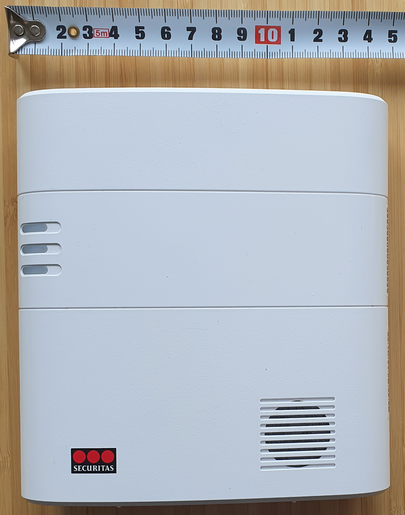
\includegraphics[height=2.15in]{images/main-panel.png}
        \caption{Main Panel}
        \label{fig:main-panel}
    \end{subfigure}%
    ~
    \begin{subfigure}[t]{0.33\textwidth}
        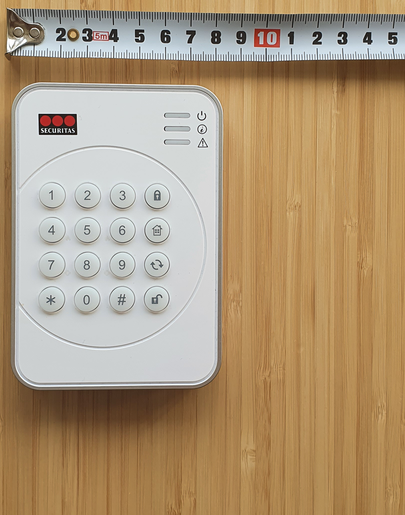
\includegraphics[height=2.15in]{images/keypad.png}
        \caption{Remote Keypad}
        \label{fig:remote-keypad}
    \end{subfigure}%
    ~
    \begin{subfigure}[t]{0.33\textwidth}
        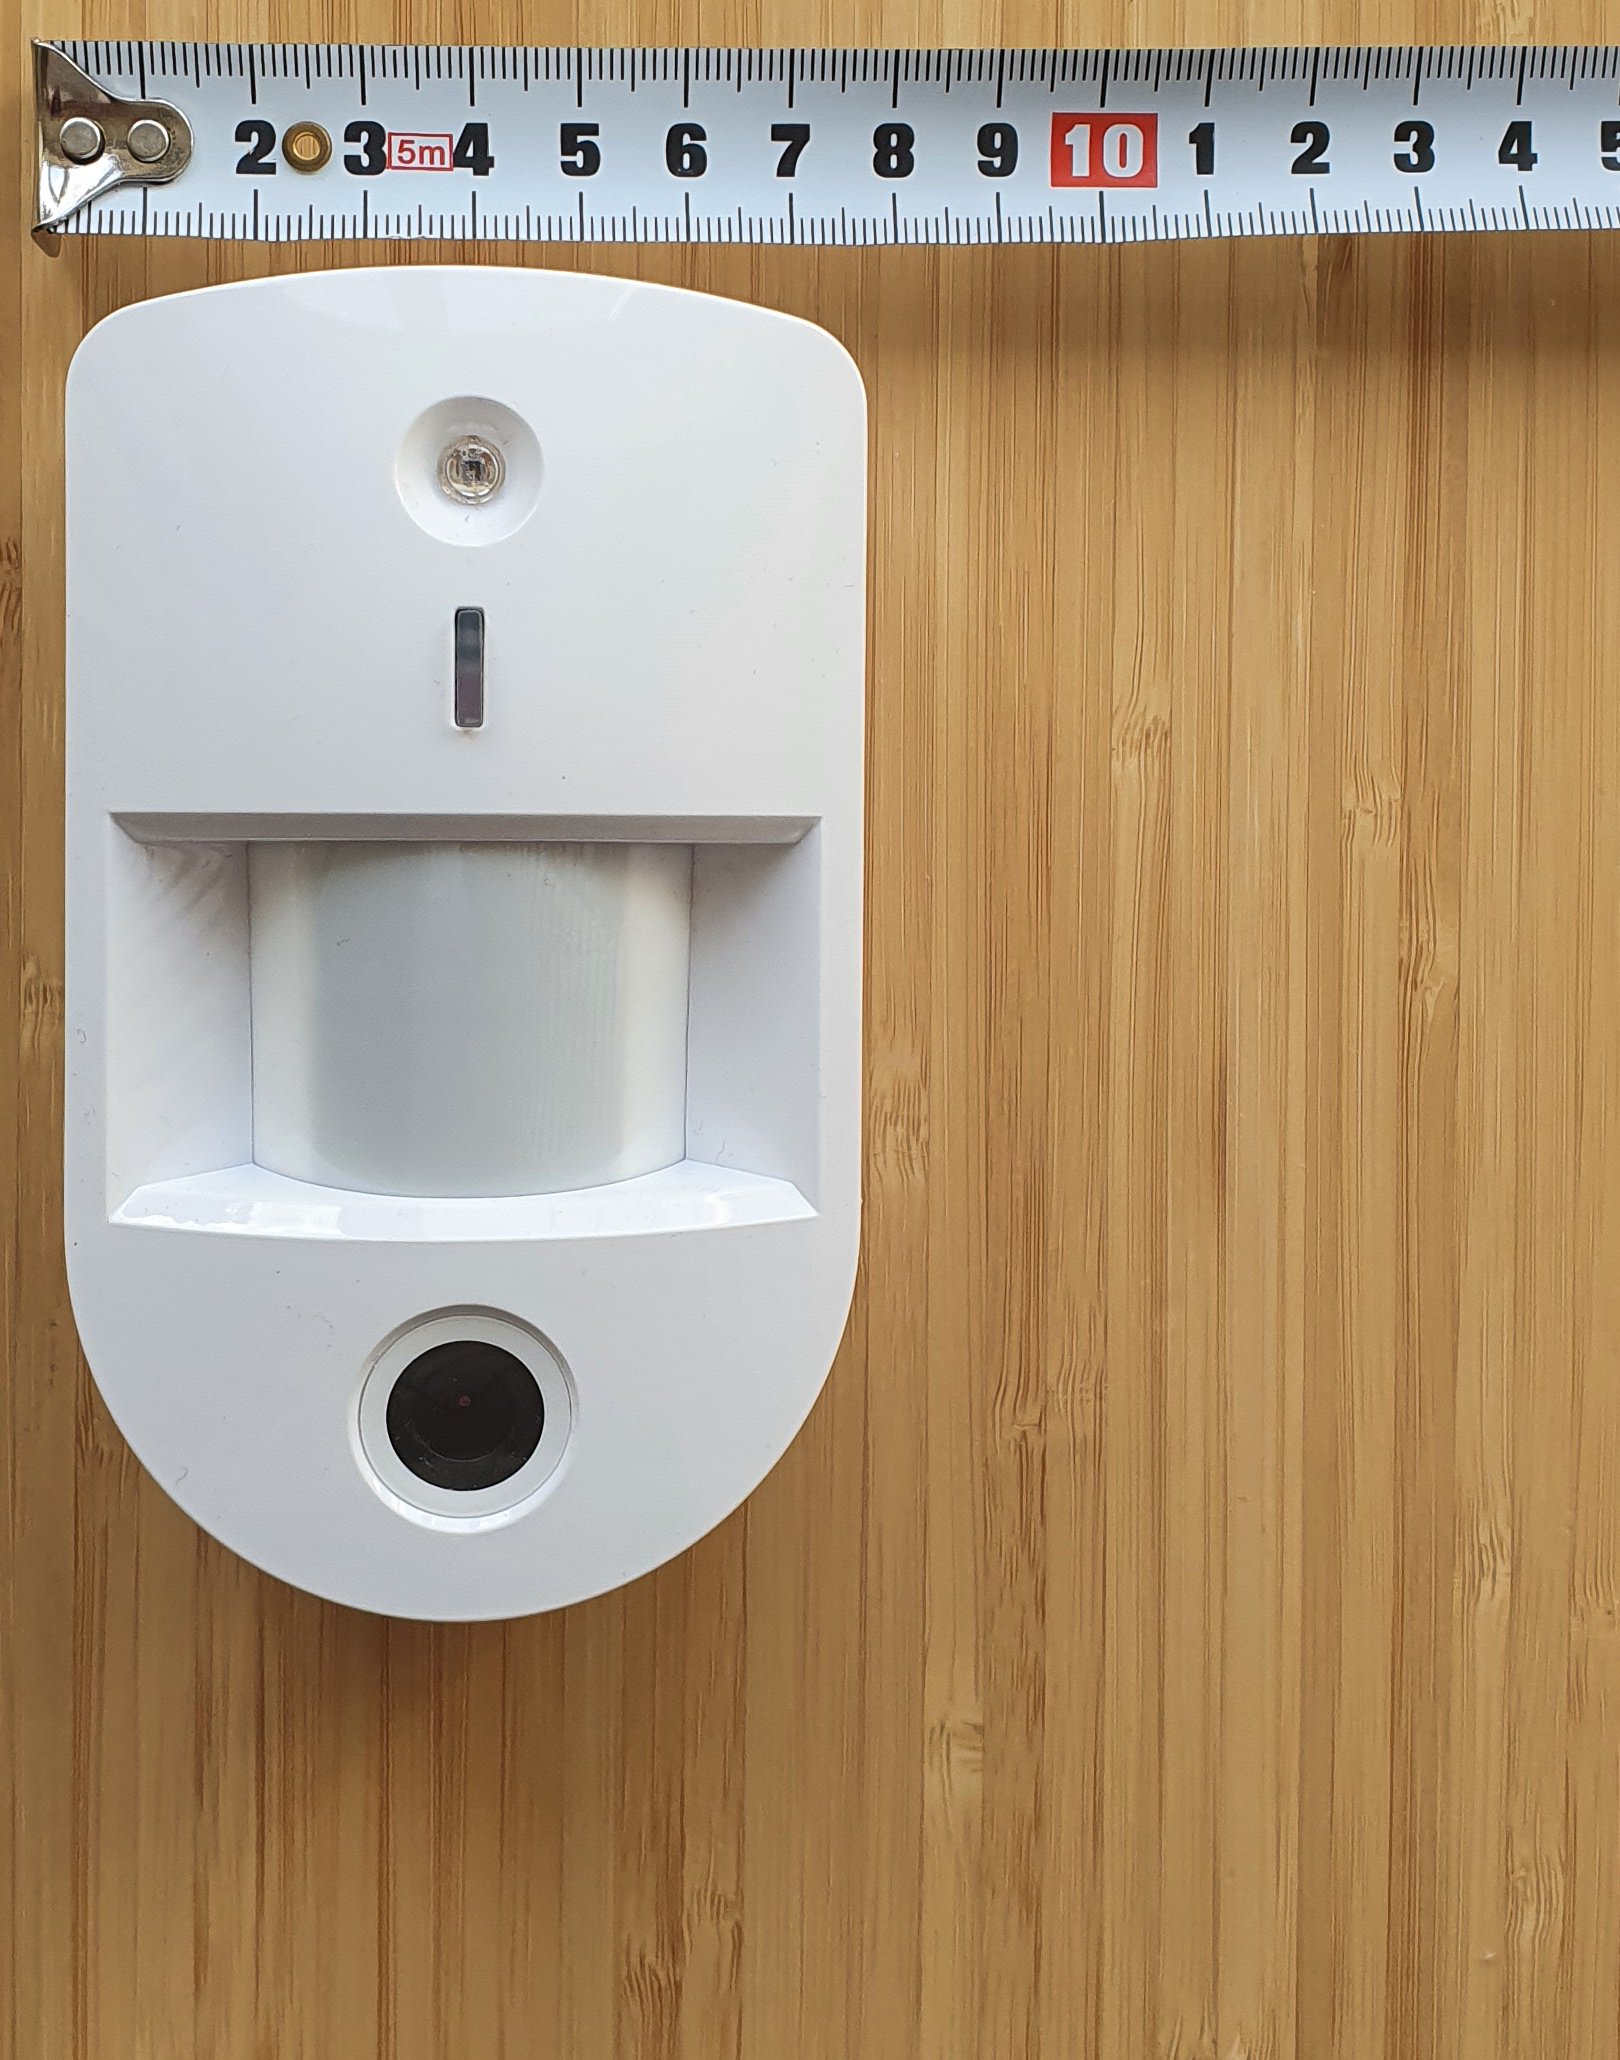
\includegraphics[height=2.15in]{images/camera.png}
        \caption{Motion Detection Camera}
        \label{fig:motion-camera}
    \end{subfigure}
    
    \begin{subfigure}[t]{0.33\textwidth}
        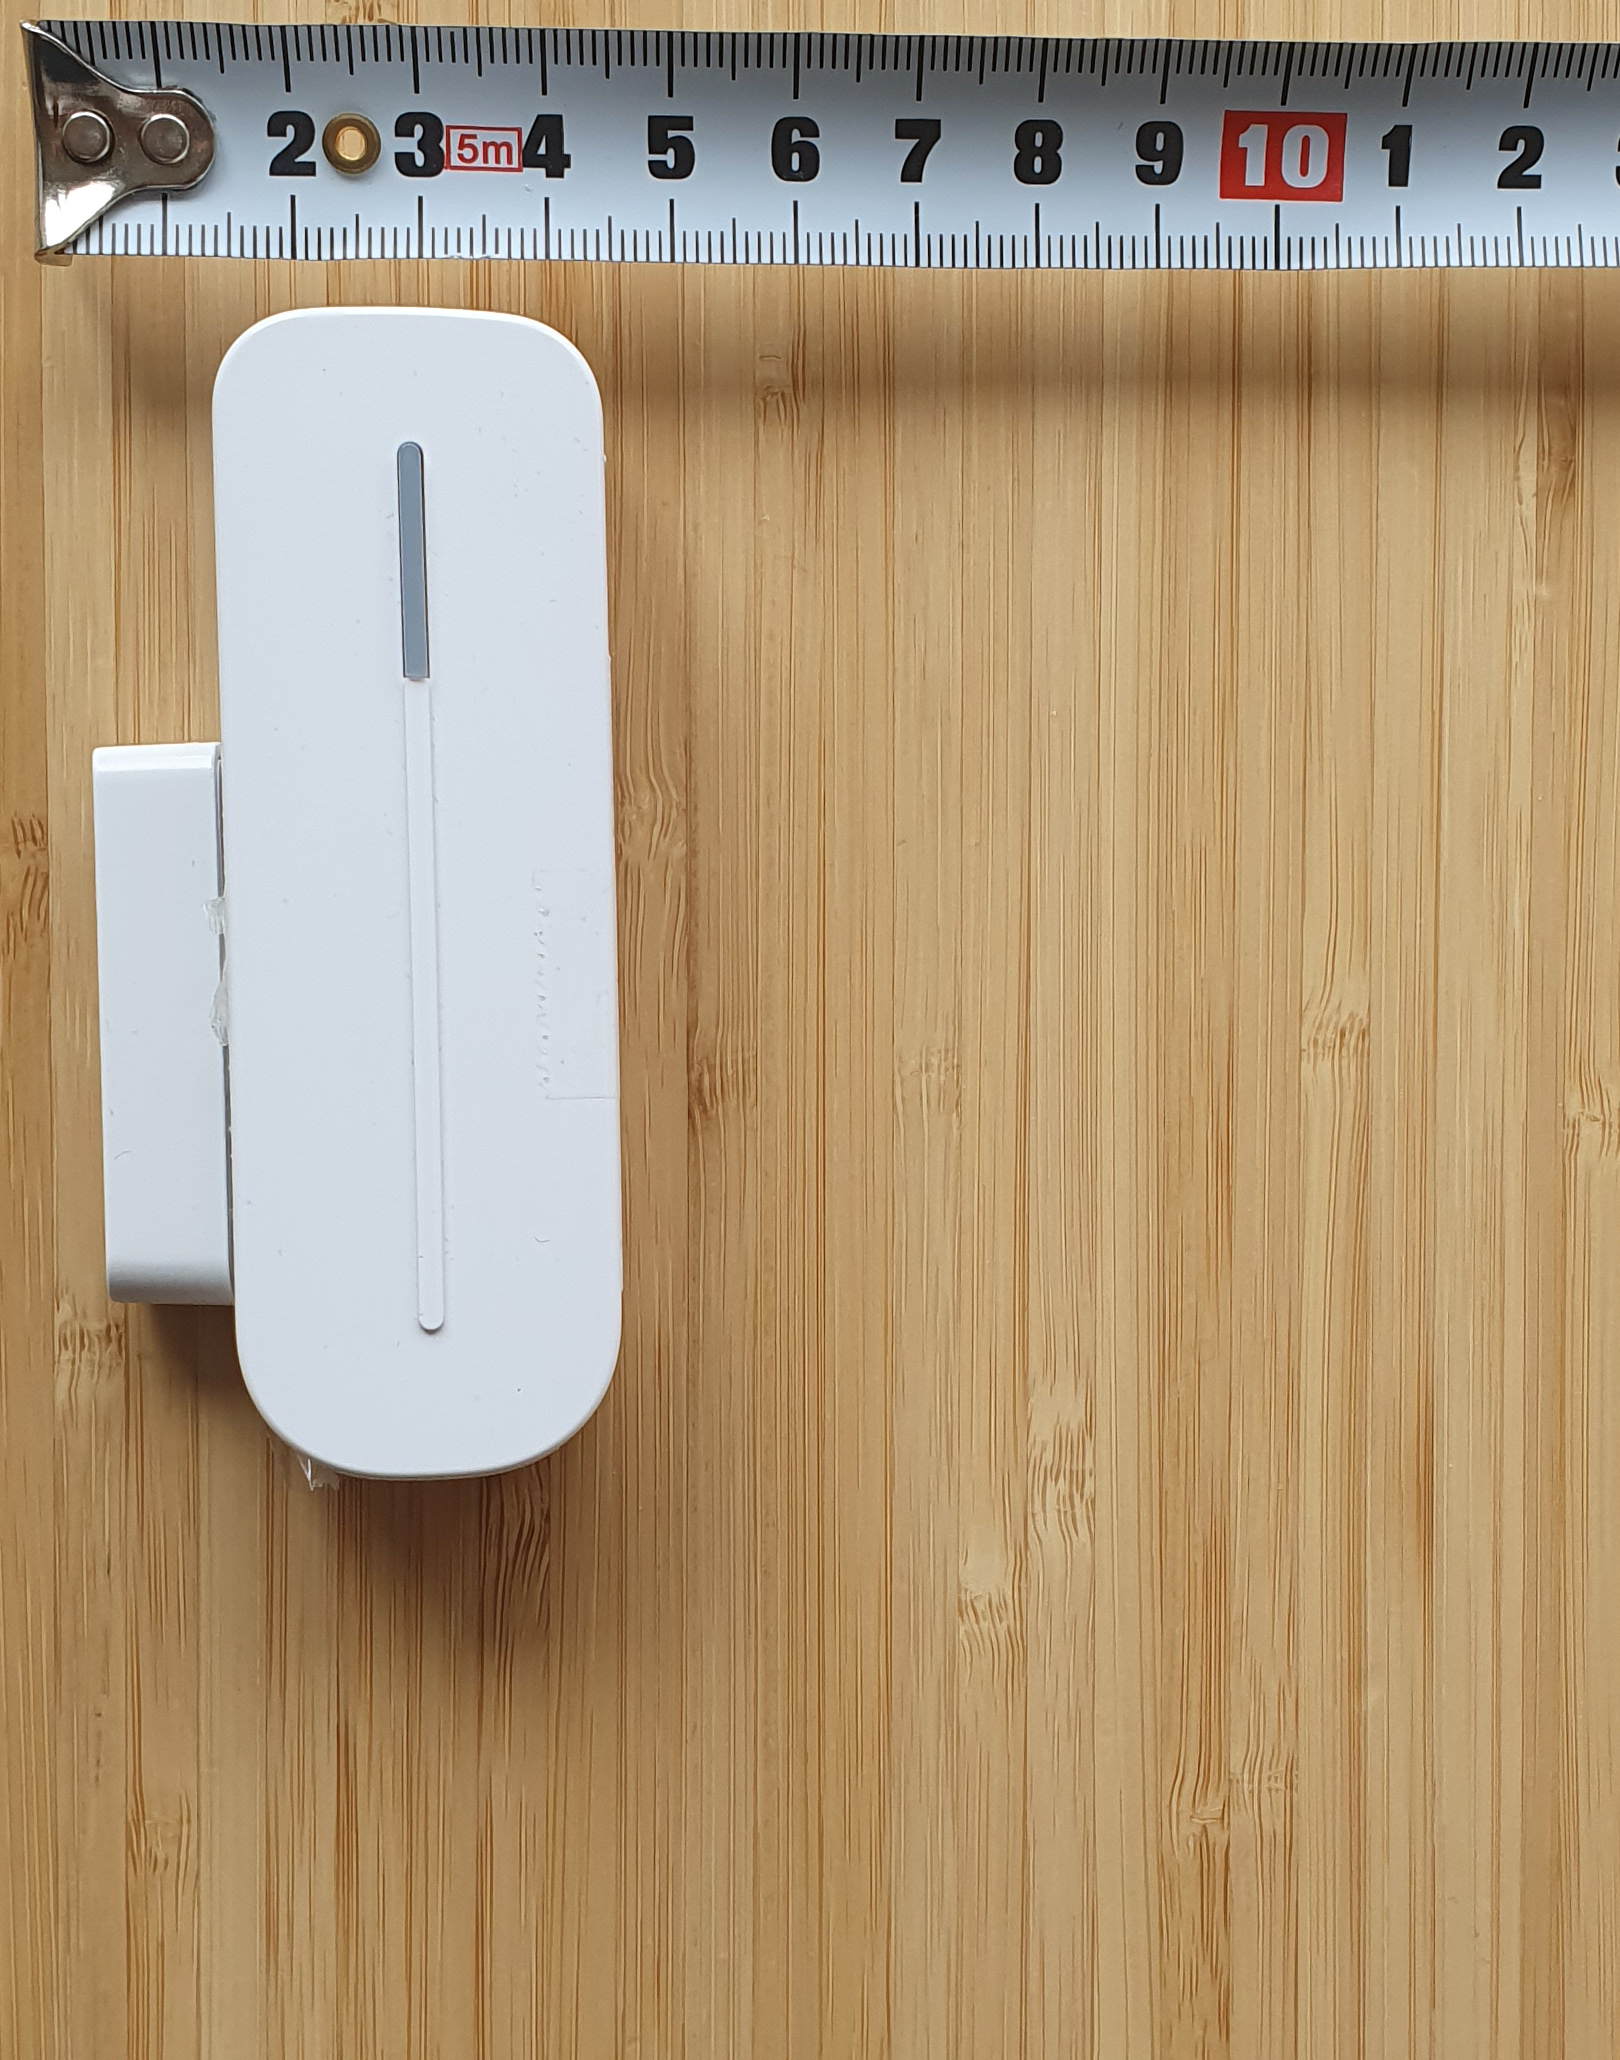
\includegraphics[height=2.15in]{images/door-contact.png}
        \caption{Door Contact Sensor}
        \label{fig:door-contact}
    \end{subfigure}%
    ~
    \begin{subfigure}[t]{0.33\textwidth}
        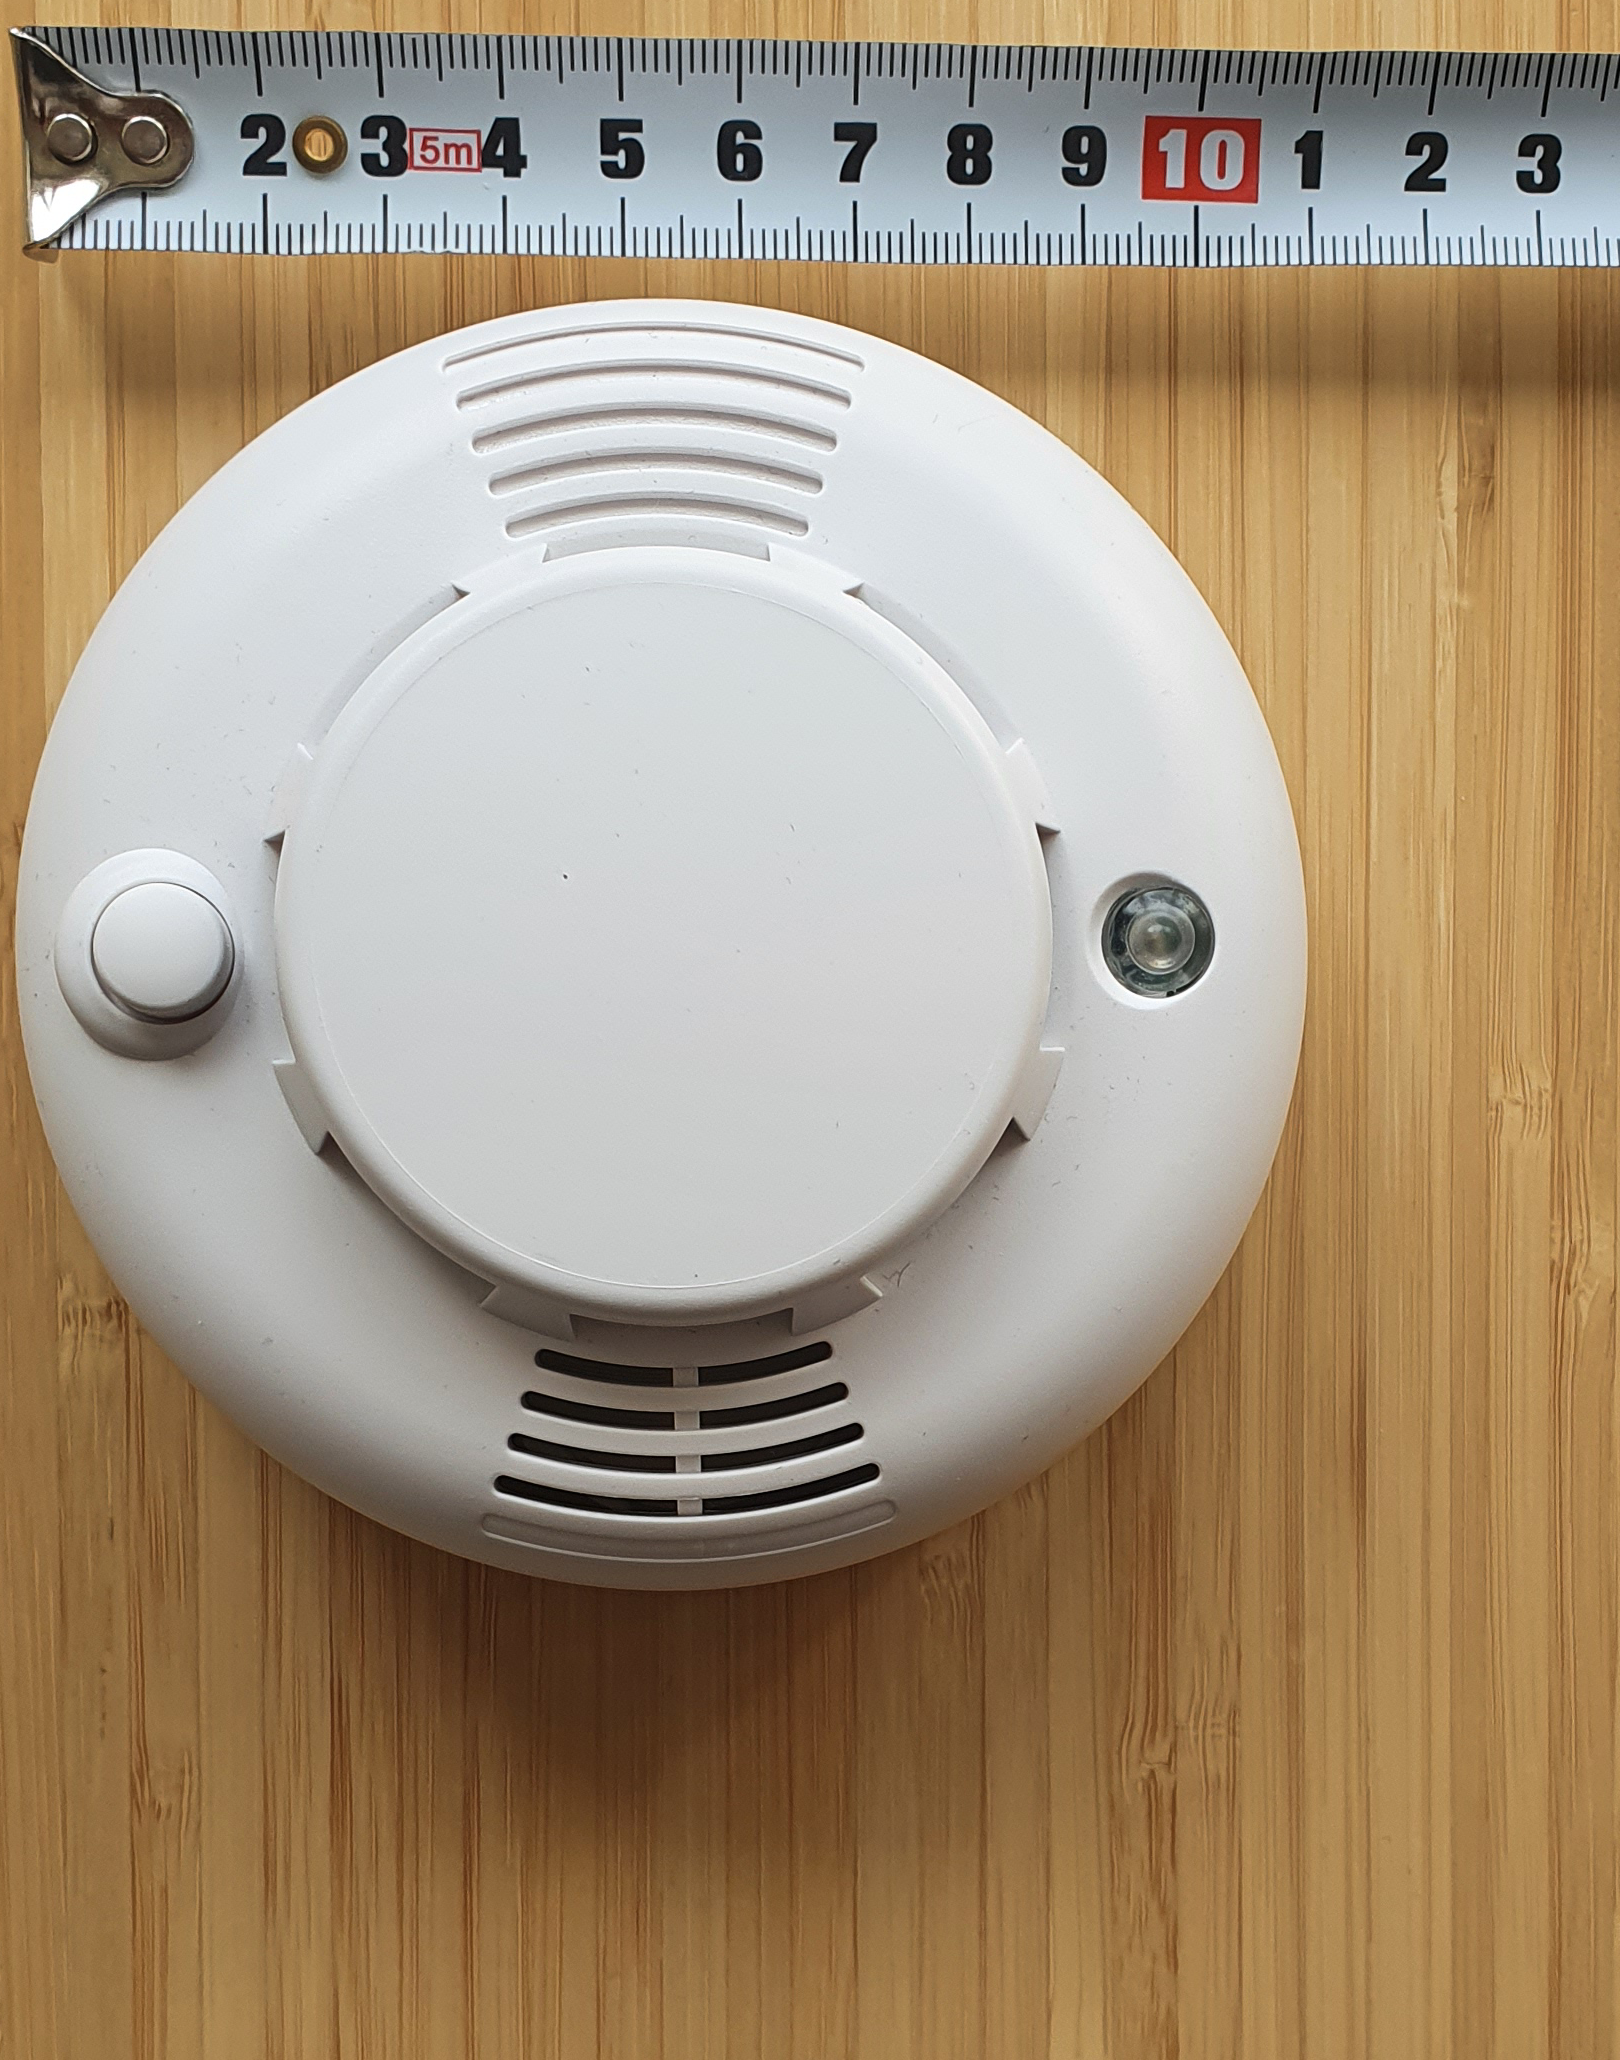
\includegraphics[height=2.15in]{images/smoke-detector.png}
        \caption{Smoke Detector}
        \label{fig:smoke-detector}
    \end{subfigure}
    \caption{The hardware components of the system}
    \label{fig:hardware-components}
\end{figure}
\subsubsection{Main Panel}
\textbf{Model number:} HSGW-G8-3G/LTE-ZW-F1 433/868 \\
\textbf{FCCID:} GX9HSGWF1919 \\
The main panel, see figure \ref{fig:main-panel}, is the \textit{"brains"} of the system so to speak. It handles communication with all other hardware devices as well as external servers. Through radio wave communication it talks to the other hardware peripherals of the system. It uses 3G telecommunication to talk to the external servers.

\subsubsection{Remote Keypad}
\textbf{Model number:} KPT-23-EL-F1 \\ % could also be KPT-23N-EL-F1, not sure
\textbf{FCCID:} GX9KPF1 \\ % This says KPF but it looks the same..
The remote keypad is a 16 button keypad used to arm and disarm the system using a personal 4 digit pin. See figure \ref{fig:remote-keypad}. This device talks to the main panel over radiowave communication.

\subsubsection{Motion Detection Camera}
\textbf{Model number:} VST-862-F1 \\
\textbf{FCCID:} GX9862 \\
This device, see figure \ref{fig:motion-camera}, features an infra-red sensor to detect motion, and a camera to survey the location. When triggered the device takes two pictures which are sent to the main panel. It is not a surveillance camera, meaning it does not continuously take pictures. The camera is only active when motion is detected and the alarm is triggered, presumably to save power.

\subsubsection{Door Contact Sensor}
\textbf{Model number:} DC-23-F1 \\
\textbf{FCCID:} GX9DC23 \\
This device, see figure \ref{fig:door-contact}, senses when a door or window is opened. A small external magnet is placed on the door/window close to the device. When these are separated the device is triggered and communicates with the main panel over radio wave communication.

\subsubsection{Smoke Detector}
\textbf{Model number:} SD-8EL \\
\textbf{FCCID:} GX9SD8ELF1919 \\
This device is a smoke detector, see figure \ref{fig:smoke-detector}. It communicated with the main panel over radio-waves and also includes a siren which triggers when it detects smoke.

\subsection{Software} \label{ch:system:software}
This section details the three software entry points from where the user can control the alarm and view it's state.

\subsubsection{Web portal}
The web portal is a webpage created by the American company \textit{Alarm.com}, see figure \ref{fig:company-structure}, hosted at \url{https://www.alarm.com/web/system/}. From the landing page, see figure \ref{fig:web-landing-page}, the user can see the following:
\begin{itemize}
    \item If the system has any issues. This can be seen in the \textit{System OK} box in figure \ref{fig:web-landing-page}.
    \item The state of each sensor of the system, like the door contact sensor (see figure \ref{fig:door-contact}).
    \item The arm/disarm state of the system.
    \item The latest photograph taken by the motion detection camera (see figure \ref{fig:motion-camera}).
\end{itemize}
Crucially, from the landing page, the user can also easily arm or disarm the system, see figure \ref{fig:web-arming}. Beyond this, the user can also see a list of recent activity in the system, change users personal four digit pin codes, and create new users.

\begin{figure}[!ht]
    \centering
    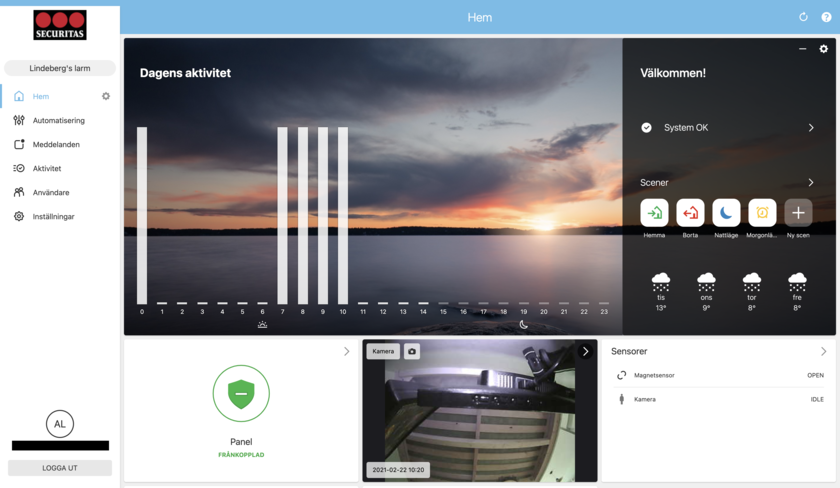
\includegraphics[width=\textwidth]{images/landing-page-web.png}
    \caption{The web portal landing page.}
    \label{fig:web-landing-page}
\end{figure}
\begin{figure}[!ht]
    \centering
    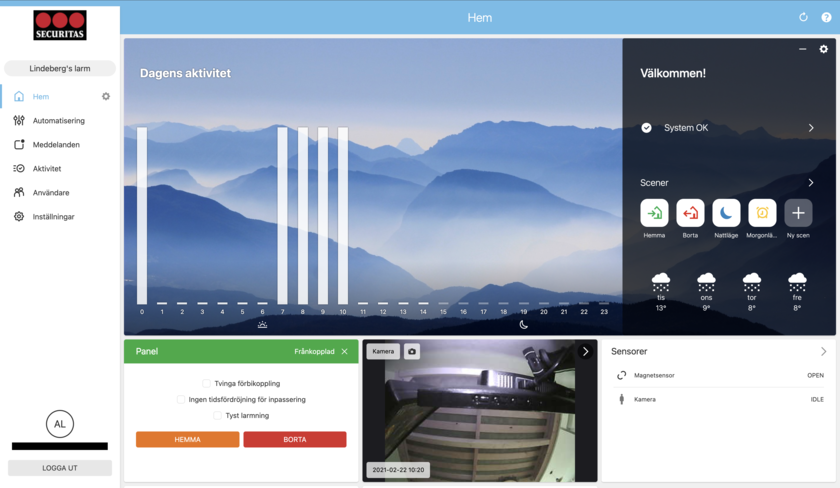
\includegraphics[width=\textwidth]{images/arming-web.png}
    \caption{Arming the alarm from the web portal.}
    \label{fig:web-arming}
\end{figure}

\subsubsection{Mobile application}
The system can also be controlled and administrated via a mobile application, free to download via the \textit{Google Play Store}, called \textit{Securitas Connect}\footnotelink{https://play.google.com/store/apps/details?id=com.alarm.alarmmobile.android.securitas}{2021-03-30}. As explained previously, while the application is branded by Securitas, it is created and developed by \textit{Alarm.com}. The interface very closely resembles the web portal, see figure \ref{fig:mobile-landing-page}, and offers identical functionality, see figure \ref{fig:mobile-landing-page}.
\begin{figure}[!ht]
    \centering
    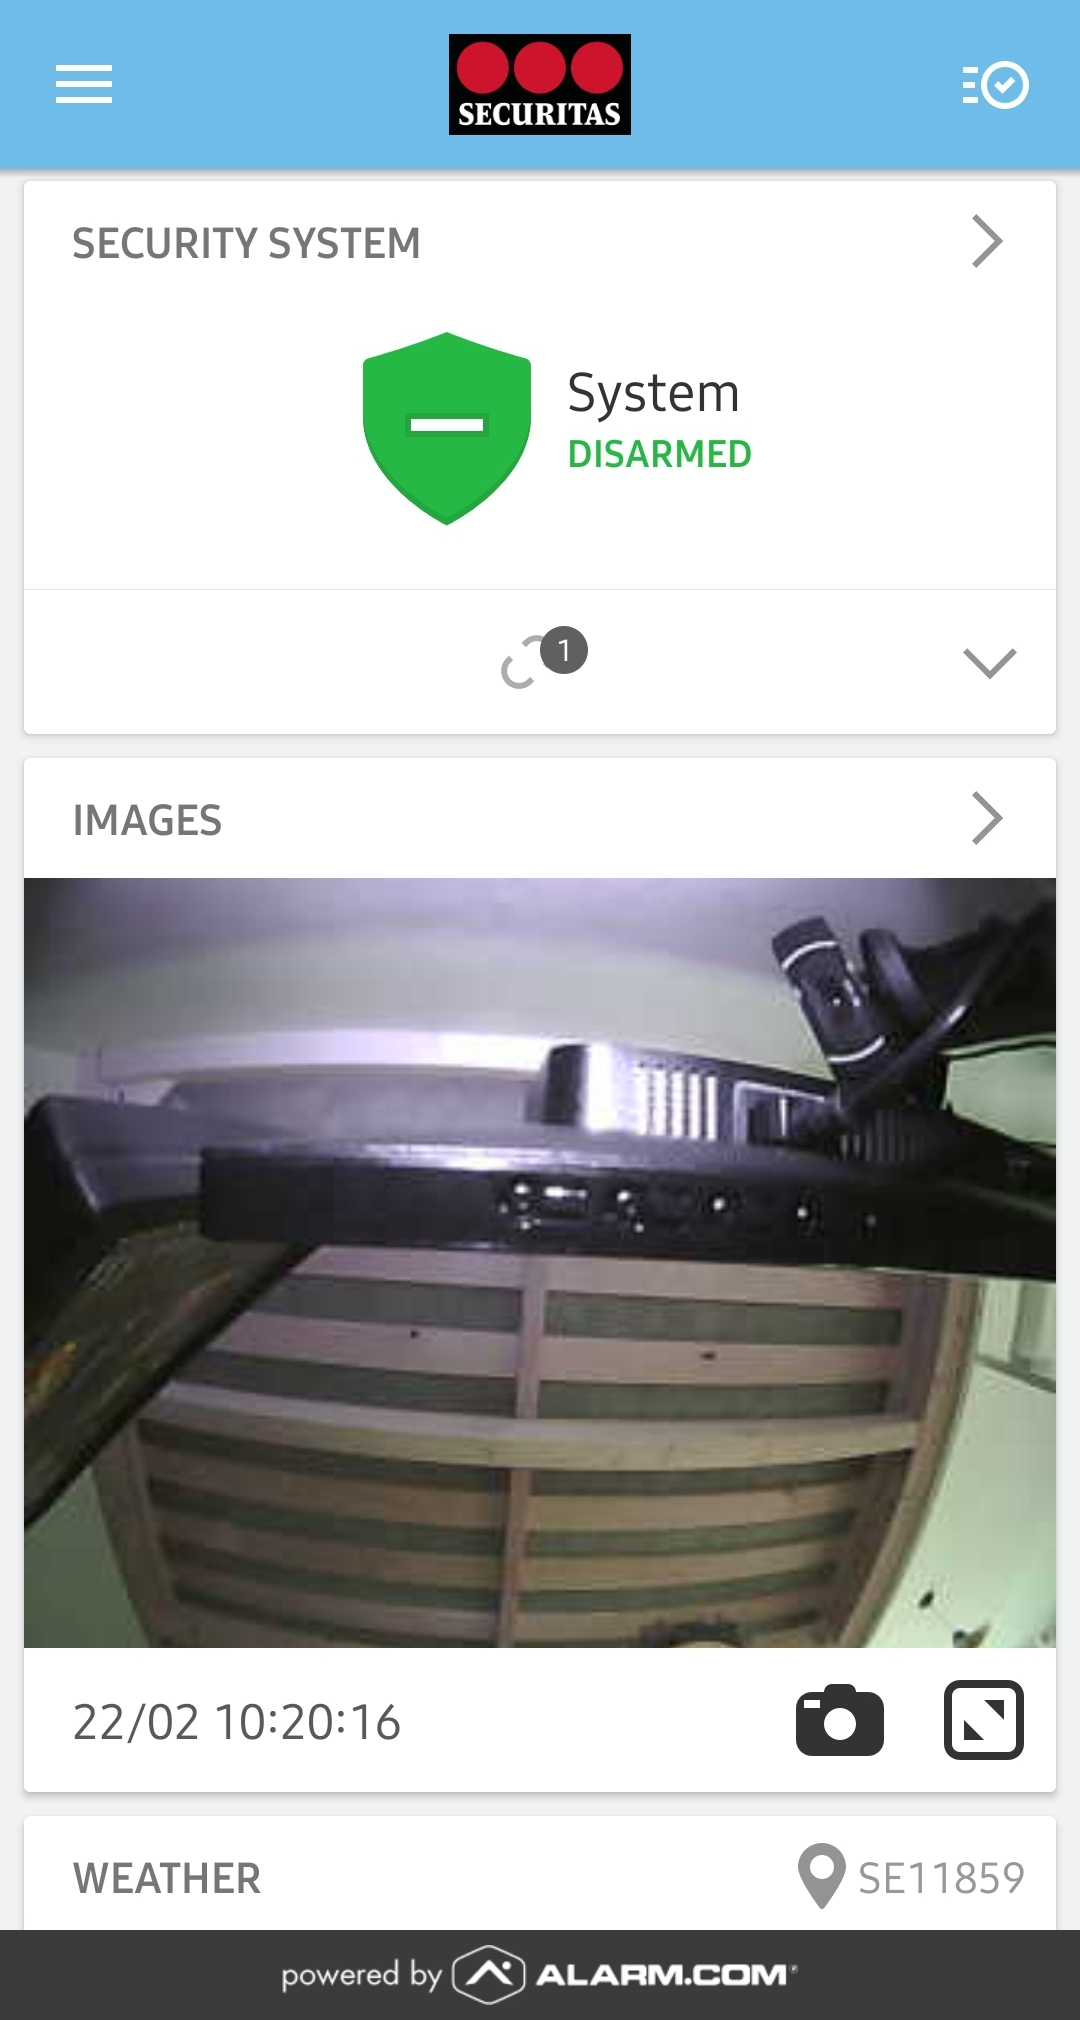
\includegraphics[width=0.5\textwidth]{images/mobile-landing-page.jpg}
    \caption{The android mobile app landing page.}
    \label{fig:mobile-landing-page}
\end{figure}

\subsubsection{Local web admin page}
Beyond the two applications created by \textit{Alarm.com} described above, the main panel (see figure \ref{fig:main-panel}) hosts a web server on the local network. This feature is undocumented, and is presumably not meant to be used or found by the regular, non-tech-savvy consumer. The page is not hosted on any domain name, as far as the author is aware, and instead has to be accessed directly via the main panels local IP address on port 80. The landing page of this web server, see figure \ref{fig:local-landing-page}, is quite simple and shows some basic information about the system such as the MAC address, IMEI number of the cellular communication, etc. Beyond that, the site only has two actions the user can do. One is to perform a "\textit{Phone Test}", to presumably test the connection to the mobile 3G network, and the other is a "\textit{Network Scan}". Once the network scan has completed, the page shows a list of all reachable telecommunication towers, see figure \ref{fig:local-network-scan}.
\begin{figure}[!ht]
    \centering
    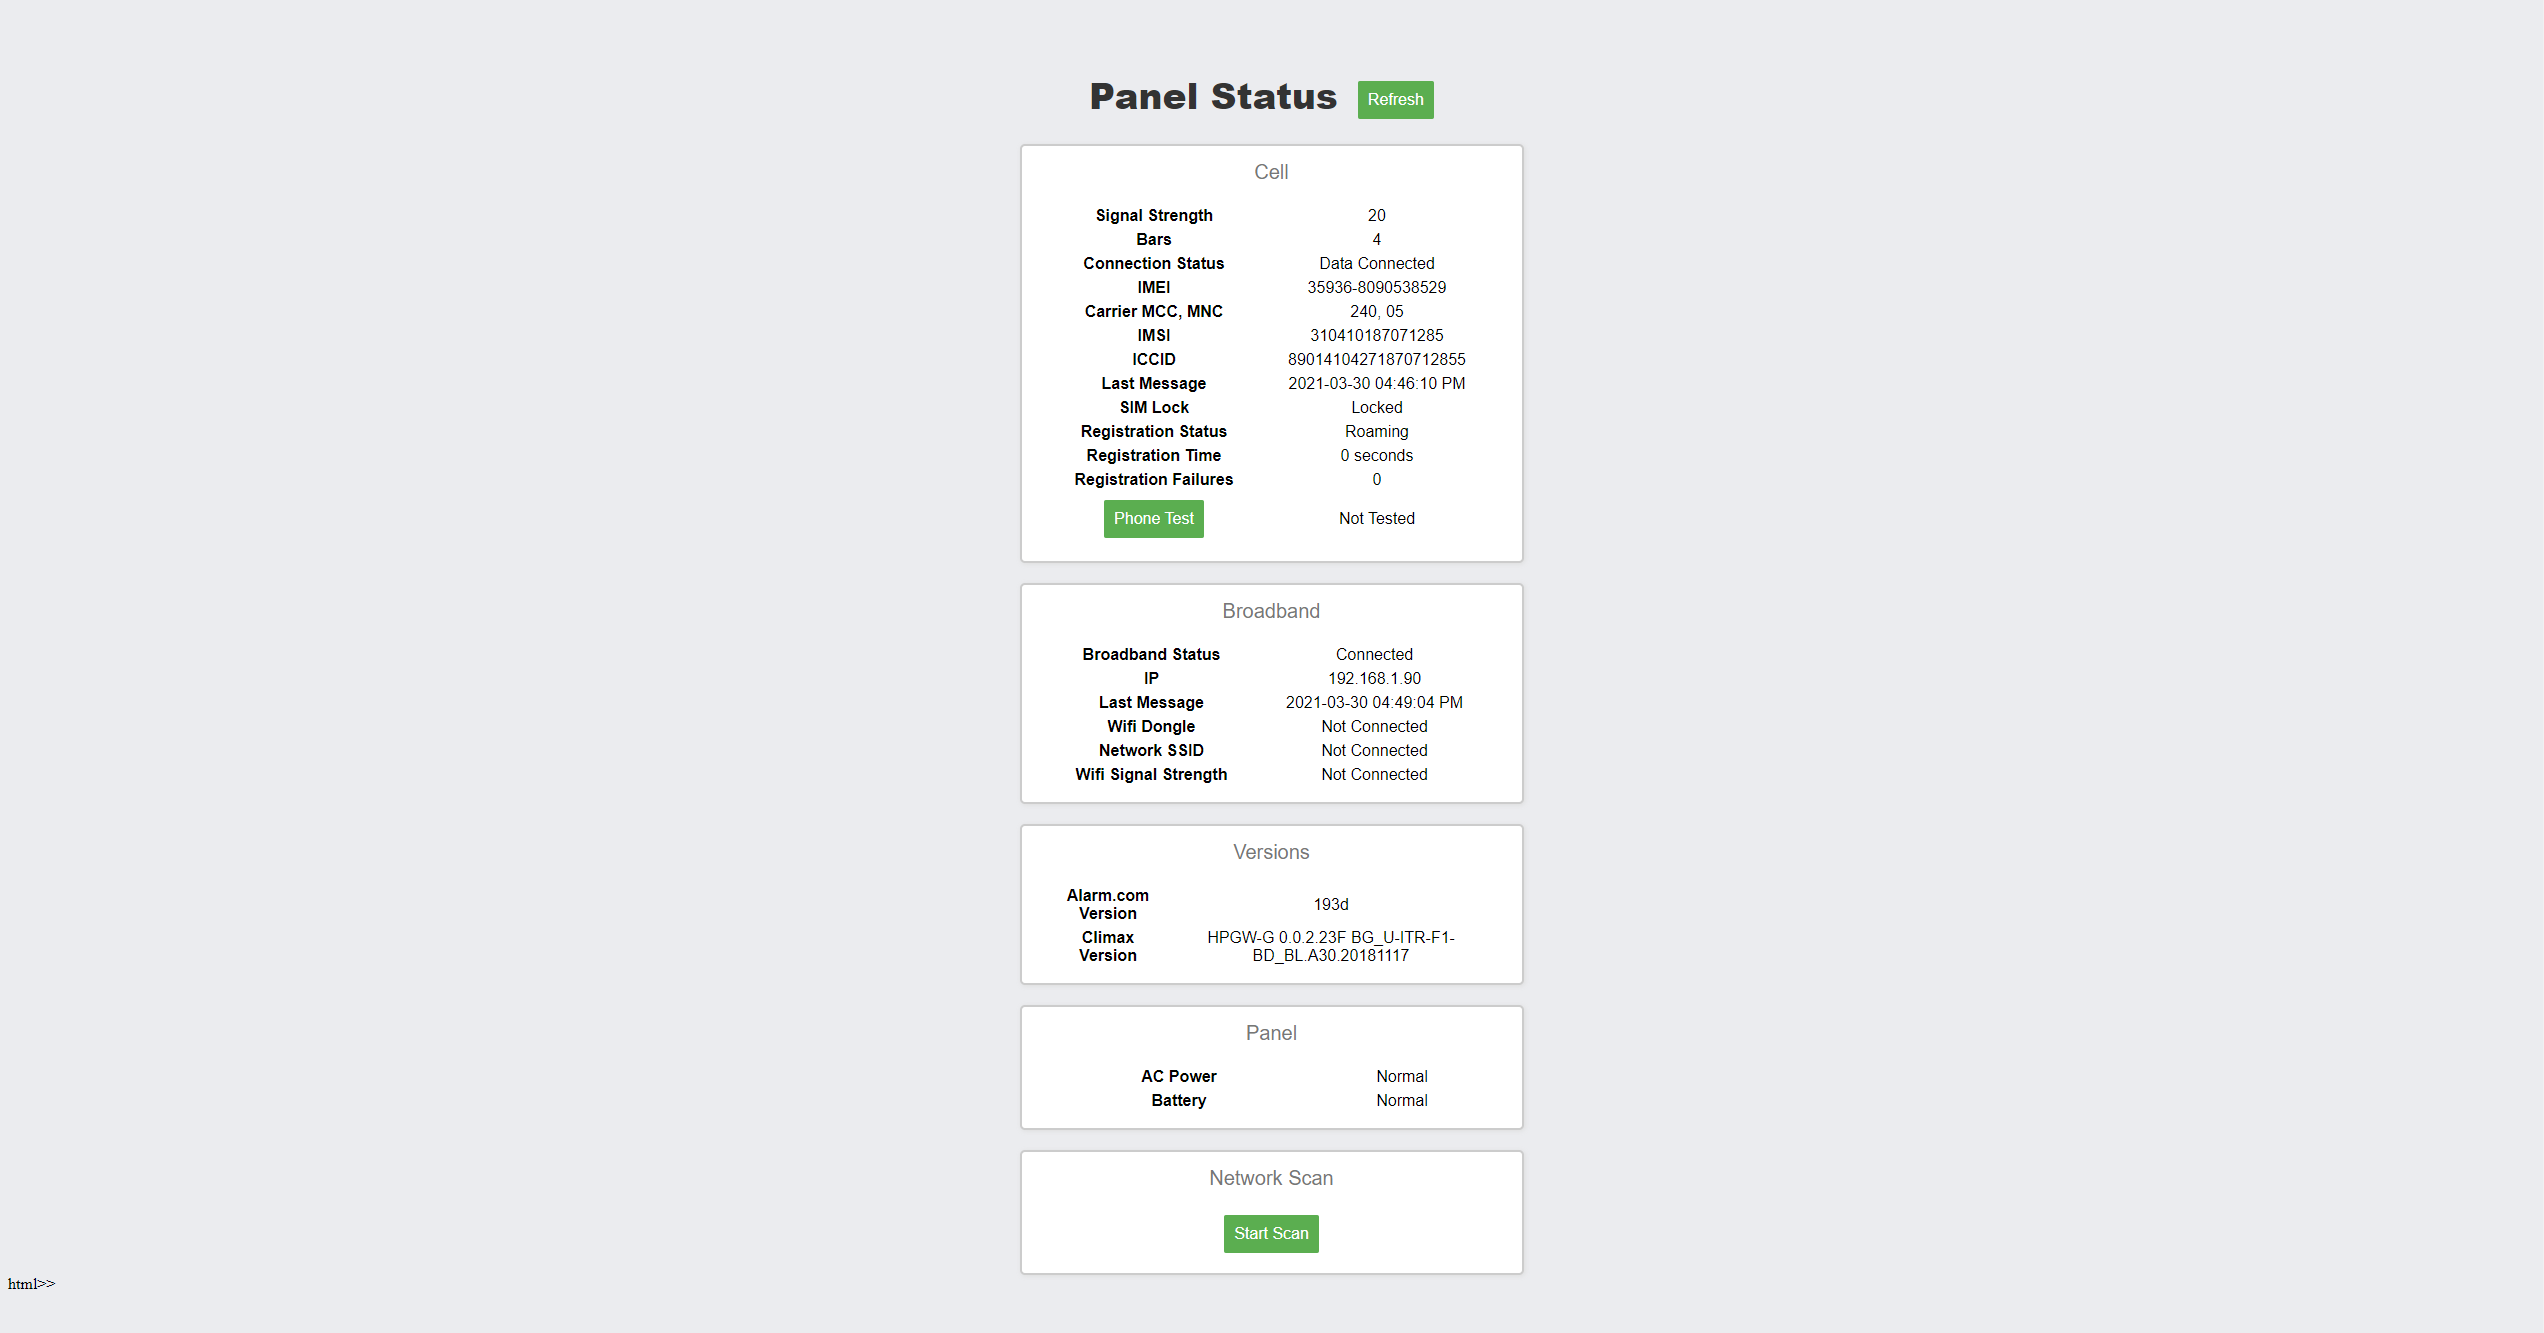
\includegraphics[width=\textwidth]{images/local-landing-page.png}
    \caption{The local web server's landing page.}
    \label{fig:local-landing-page}
\end{figure}
\begin{figure}[!ht]
    \centering
    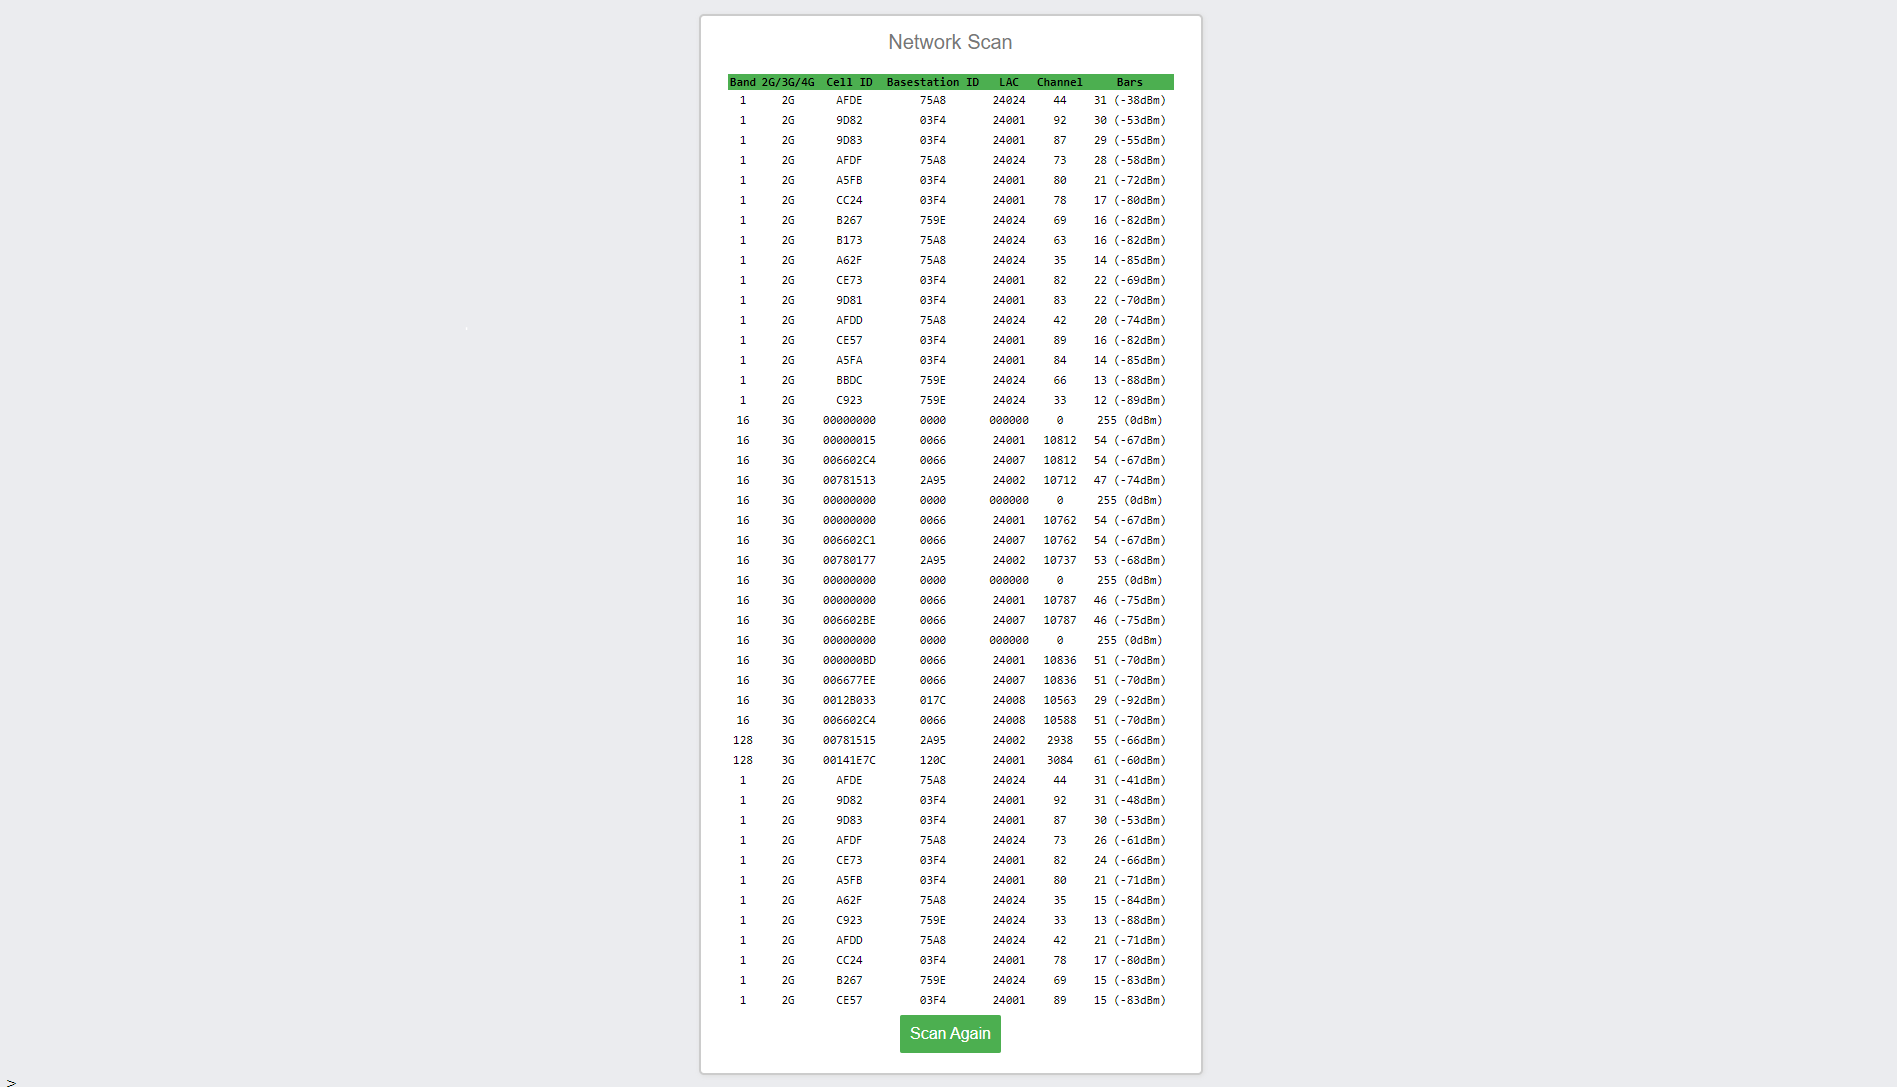
\includegraphics[width=\textwidth]{images/local-network-scan.png}
    \caption{A mobile network scan from the local web server.}
    \label{fig:local-network-scan}
\end{figure}
\begin{figure}[!ht]
    \centering
    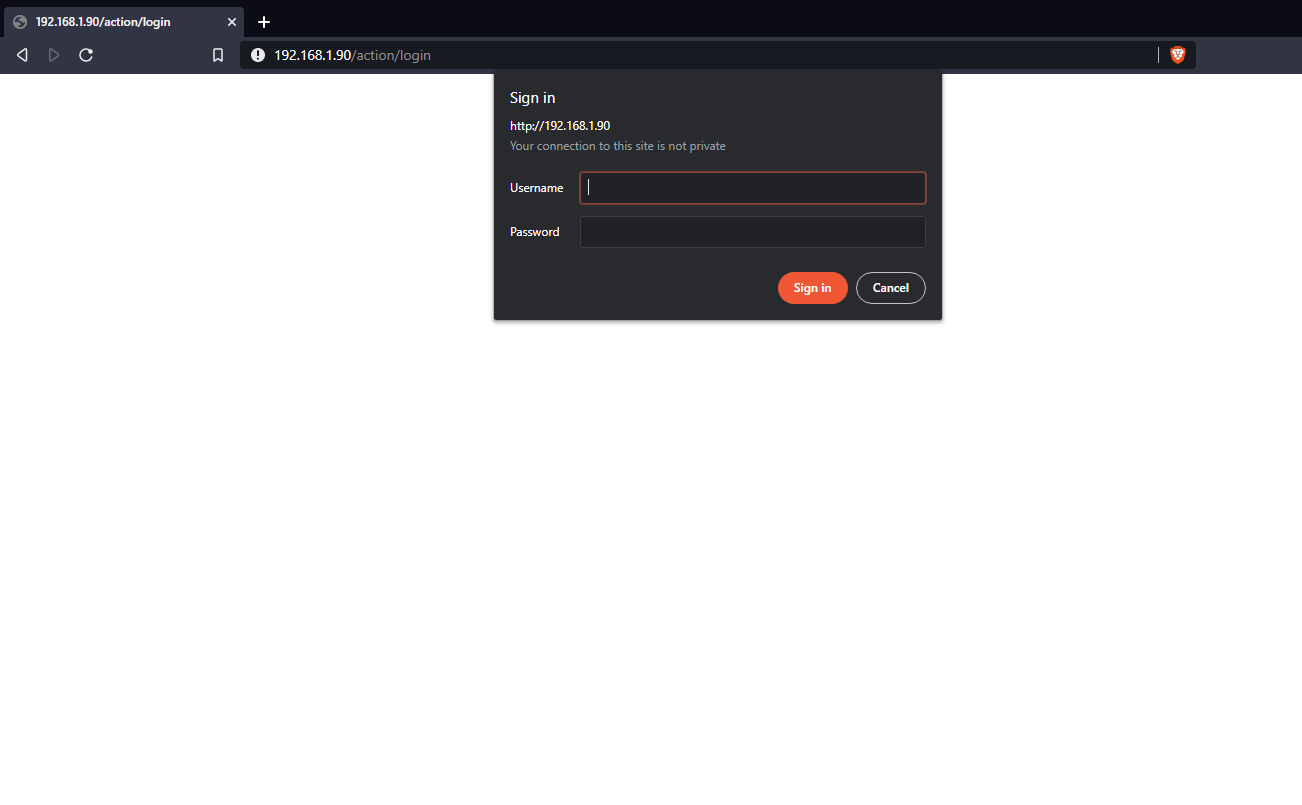
\includegraphics[width=\textwidth]{images/local-login-page.png}
    \caption{The local web server's HTTP Basic Auth login page.}
    \label{fig:local-login-page}
\end{figure}
\begin{figure}[!ht]
    \centering
    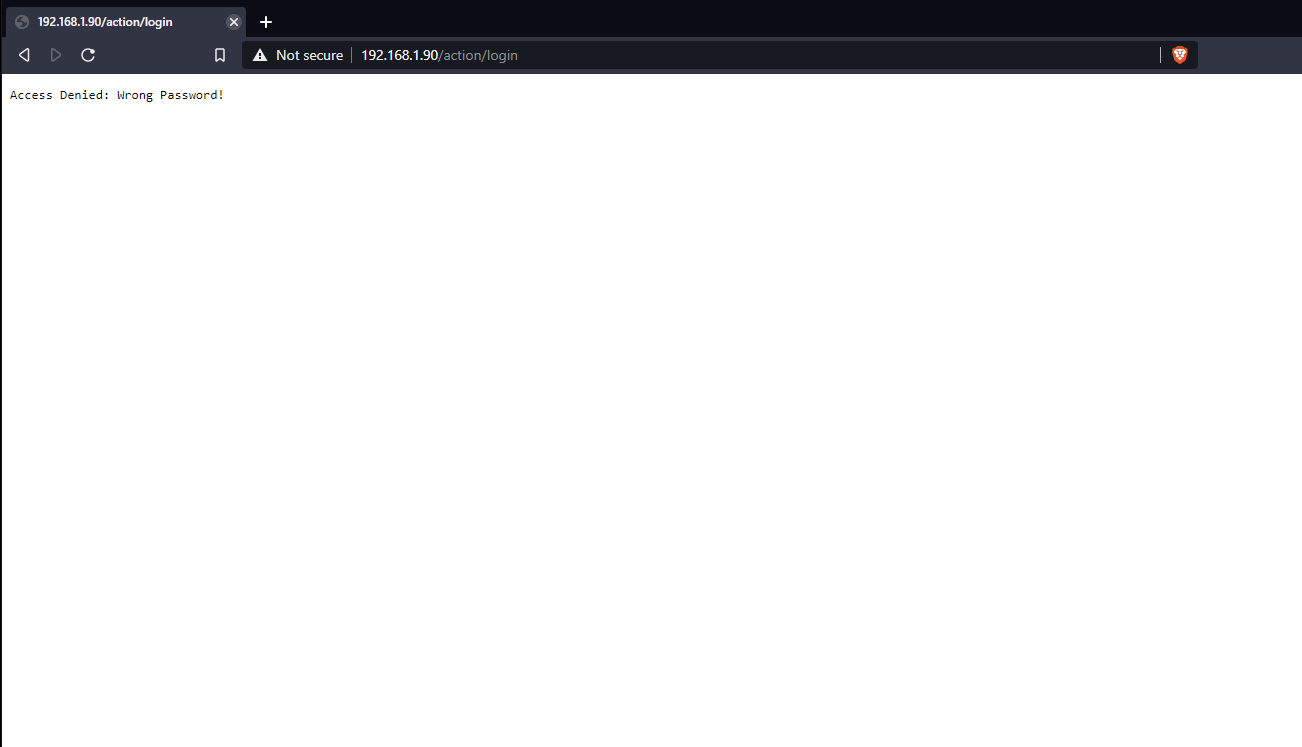
\includegraphics[width=\textwidth]{images/local-login-denied.png}
    \caption{A failed login attempt on the local web server.}
    \label{fig:local-login-denied}
\end{figure}
Additionally, the web page features an undocumented login page on the path \texttt{/action/login}, see figure \ref{fig:local-login-page}. This page lets the user authenticate using \textit{HTTP Basic auth}. The credentials here are not tied to the users account on the aforementioned web portal or mobile applications. Presumably this is purely meant as a backdoor for \textit{Climax Technology} for debugging purposes, and not meant to be used by the user of the system. If wrong credentials are entered the user is presented with a static message, saying they have the wrong password (see figure \ref{fig:local-login-denied}), providing zero additional functionality.
\chapter{Related work} \label{ch:related-work}
This chapter describes identified related works done in the same area and specifically against the hardware used in the system. The OWASP IoT Top 10 is described as well as its relevance to this report. Additionally, the ETSI EN 303 645 standard for development of secure IoT products is covered. Regarding the system under consideration, very little has been published regarding the cybersecurity of this specific IoT system, as far as the author is aware. However, two sources that explore systems based on the hardware from the same manufacturer, Climax Technology, have been identified. Additionally, a student thesis was done on a similar system but from a different manufacturer. These are presented below. Lastly, two talks on RF hacking are presented. These present common techniques in RF hacking and what types of vulnerabilities are common in RF communication.

\section{OWASP IoT Top 10} \label{ch:related-work:owasp}
The OWASP top 10 for web vulnerabilities is one of the most used sources of the most common web vulnerabilities \cite{owasp-www-top10}. The OWASP Foundation, the publisher of the report, claims it is \enquote{globally recognized by developers as the first step towards more secure coding}\footnotelink{https://owasp.org/www-project-top-ten/}{2021-05-21}. OWASP also compiles and publishes a list of the top ten most common vulnerabilities for specifically IoT systems \cite{owasp-iot-top10}. The latest revision was released in \citeyear{owasp-iot-top10}. This list is highly relevant to this report as the system in question is an IoT system. In this thesis, this list was used to identify and determine the most important threats to investigate. The top ten vulnerabilities for IoT systems according to OWASP's report are the following, in order of importance:
\begin{enumerate}
    \item \textbf{Weak, Guessable, or Hardcoded Passwords}. This includes passwords that can be easily brute-forced, are publicly available, or unchangeable. Famously the MIRAI botnet, which mostly included IoT devices, managed to recruit over half a million devices to its botnet by testing just 60 default credentials \cite{understanding-mirai}.
    
    \item \textbf{Insecure Network Services}. Often unneeded network services will be left open on IoT devices, even after they are shipped to customers. Commonly, these are used during development but are never removed when the device is shipped. An example is open telnet services or ssh being left open, leaving a backdoor open for the manufacturer. However, as a consequence, these network services open the device up to a whole slew of potential vulnerabilities. Often they are also completely unnecessary for the functionality of the IoT system. A real-world example of this is again the MIRAI botnet, which scanned IP ranges for devices with telnet services hosted on port 21 or 2121 \cite{understanding-mirai}.
    
    \item \textbf{Insecure Ecosystem Interfaces}. Many IoT systems are much more than just the device itself. There is often an entire infrastructure behind it to control and interact with the system, such as a mobile application or a website, with an accompanying backend API server. Vulnerabilities anywhere in this ecosystem can lead to the security of the IoT device itself being compromised.
    
    \item \textbf{Lack of Secure Update Mechanism}. To add new features and to fix security issues, updating the firmware of IoT devices is often unavoidable. However, over-the-air (OTA) firmware updates add an additional attack vector and can introduce many potential security issues. This can include the device not validating the firmware it receives, delivering the firmware unencrypted in transit, a lack of a mechanism to prevent rolling back changes, and a lack of notifications of security changes due to updates.
    
    \item \textbf{Use of Insecure or Outdated Components}. This means using old versions of libraries and components that themselves are vulnerable. These can then in turn compromise the security of the system as a whole. This can include everything from insecure versions of operating systems, insecure customization of the OS, third-party software, and insecure hardware components from higher up in the supply chain.
    
    \item \textbf{Insufficient Privacy Protection}. This refers to the user's personal information being stored in an insecure way. Either on the IoT system itself or in the larger ecosystem.
    
    \item \textbf{Insecure Data Transfer and Storage}. Lack of encryption or proper access control, both in transit and in storage. This can, once again, be both on the IoT device and anywhere else in the larger ecosystem.
    
    \item \textbf{Lack of Device Management}. This includes lack of secure asset management, update management, secure decommissioning of the system, proper monitoring of the system, as well as capabilities to respond to a security issue.
    
    \item \textbf{Insecure Default Settings}. This refers to the device being sold with insecure default settings. Often the user is never prompted or encouraged to change these insecure defaults.
    
    \item \textbf{Lack of Physical Hardening}. During development, debug hardware interfaces are used. However, a common vulnerability is not removing these before shipping the product. This can include open JTAG or UART interfaces on the circuit board, allowing for the extraction of the firmware or even terminal access to the system over a serial interface. Often these vulnerabilities require physical access to the system. However, they can be used to extract valuable information which can help an attacker in developing remote exploits.
\end{enumerate}
Note that some of these threats were not considered in this report. Some of these fall under the delimited areas described in section \ref{ch:intro:delimitations}, such as number three for example. Others were not considered simply due to time constraints. However, the OWASP IoT top 10 list was the basis for the identified threats against the system, along with the STRIDE model described in section \ref{ch:method:stride}.

\section{ETSI EN 303 645, a standard for IoT security of consumer products} \label{ch:related-work:etsi}
The \textit{European Telecommunications Standards Institute} (ETSI) is a standardization organization within information and communication technology (ICT). It is responsible for standardizing key technologies like GSM, 3G, 4G, and 5G. One of the standards produced by ETSI is of relevance to this report. In their standard \citetitle{etsi-iot-standard}, they list 13 provisions that should be followed by manufacturers selling consumer facing IoT products \cite{etsi-iot-standard}. While following the standard is certainly not a guarantee that the system is secure, it provides a set of best practices of common security issues to avoid in IoT systems. Within the provisions are sub-provisions which will not be covered in full detail here. What follows is an overview of the 13 provisions as outlined by ETSI \cite{etsi-iot-standard}.
\begin{enumerate}
    \item \textbf{No universal default passwords}. All passwords have to be either supplied by the user or unique per device. No password should work across all devices. Additionally, they warn against schemes were the password is generated using publicly available information like the systems MAC address or WiFi SSID.
    
    \item \textbf{Implement a means to manage reports of vulnerabilities}. The manufacturer should make publicly available a process for disclosing vulnerabilities. It should include contact information for disclosing security issues and information on timelines during a disclosure process.
    
    \item \textbf{Keep software updated}. The manufacturer needs to implement a way of sending out security patches in a timely manner and make sure that this done in reaction to discovered vulnerabilities.
    
    \item \textbf{Securely store sensitive security parameters}. This could be encrypted storage or dedicated security components implemented in hardware for example. Additionally, it states that hard-coded critical security parameters in the device software should not be used.
    
    \item \textbf{Communicate securely}. Best practices in encrypted communications should be used in all communication, including using reviewed and well-tested cryptography methods.
    
    \item \textbf{Minimize exposed attack surfaces}. The standard recommends adhering to the \textit{principle of least privilege}, meaning one should aim to give each actor the minimum privilege needed to perform its function. Additionally, it states that all unused or unnecessary network and logical interfaces should be disabled. Only software services that are absolutely required for the functionality of the device should be enabled.
    
    \item \textbf{Ensure software integrity}. The system should verify its firmware and other software by using secure boot mechanisms. Additionally, if a discrepancy is noted the system should report it to the user/administrator and should not connect to any wider network than the minimum required to send the notification.
    
    \item \textbf{Ensure that personal data is secure}. Personal data in transit between devices should be properly secured using cryptography best practices.
    
    \item \textbf{Make systems resilient to outages}. Resilience should be built into the system, in terms of handling outages both in power and in network services for example. In case of a network failure the system should remain operational and keep the still viable functionality. In the event of a power loss the system should recover cleanly.
    
    \item \textbf{Examine system telemetry data}. If the system collects telemetry data it should be continuously monitored for anomalies with potential security implications.
    
    \item \textbf{Make it easy for users to delete user data}. It should be clear to the user how they can delete their data and functionality should be provided giving them access to do so. Additionally, users should be given clear notification of when their data has been deleted.
    
    \item \textbf{Make installation and maintenance of devices easy}. The installation and maintainence of the system should involve avoid decisions from the user as much as possible and follow security best practices on usability. Additionally, the manufacturer is responsible for providing adequate guidance on how to set up the system securely as well as how to check that it is set up securely.
    
    \item \textbf{Validate input data}. The system has to validate all inputs from any interface is reads from. It should never assume that the input is benign.
\end{enumerate}

\section{Related work 1: \textit{Examination of LUPUS-Electronics devices}} \label{ch:related-work:lupus}
This section details a security analysis of a very similar system, built on similar hardware from Climax Technology. The study was conducted by members of \textit{Embedded Lab Vienna for IoT \& Security} (ELVIS)\footnotelink{https://www.elvis.science/}{2021-04-09}, a project at the University of Applied Sciences Campus Vienna in Austria.

\textit{Lupus Electronics} is a German manufacturer of smart home security systems\footnotelink{https://www.lupus-electronics.de/en/}{2021-04-09}, much like \textit{Alarm.com} in the system examined in this thesis (see section \ref{ch:system:companies}). Just like Alarm.com, Lupus Electronics mostly provides the software of their system and also purchase hardware from the Taiwanese manufacturer \textit{Climax Technology}. In \citeyear{labvienna}, security researchers at ELVIS examined the security of the \textit{XT2 Plus Main Panel}. According to their report, similar hardware to the system examined in this thesis is used in that system. They reported several vulnerabilities. The most critical vulnerability they found was a Telnet server hosted on a non-standard high TCP port on the main panel. After examining the firmware of the system, and reverse engineering one of the applications, the researchers found that the password to the \texttt{root} user could be derived from a hardcoded salt and the MAC address of the panel. This meant that as long as an attacker had access to the local network, they could log in as root on the device, meaning with full privileges. With those privileges, one could easily bypass the security of the alarm completely.

While the Lupus system is not identical to the one in this thesis, much of the firmware from the hardware manufacturer is presumably the same. This assumption is strengthened by the fact that the endpoints found in the web interface of the Lupus system are the same in the thesis' system. The system under consideration in this report does not host a telnet server, however, it does host an application listening on a \textit{non-standard} high TCP port. According to their report, Climax Technology was notified about the vulnerabilities on \texttt{2019-01-09} and a firmware revision fixing the vulnerabilities was released on \texttt{2019-03-26}.

\section{Related work 2: \textit{The Internet of Things: a privacy label for IoT products in a consumer market}}
In their master thesis, author \citeauthor{iotprivacylabel} examines the design of an IoT privacy label, to help consumers recognize the security risks of the products they bring into their home \cite{iotprivacylabel}. The main objective of their thesis, while interesting, is not strictly relevant to this report. However, the thesis includes three case studies of different consumer products, one of them being highly relevant to this project. They examine the security of a home alarm system from \textit{Egardia}\footnotelink{https://www.egardia.com}{2021-04-12}, a dutch company producing smart home alarm systems. Much like \textit{Alarm.com} or \textit{Lupus Electronics} (see section \ref{ch:related-work:lupus}), Egardia are mainly responsible for the software platform and base their product on hardware from Climax Technology. While this system is not the main focus of their thesis, the author presents a short security analysis of the system and reports a few vulnerabilities. One of them, and arguably the most critical, is a replay attack vulnerability in the \gls{RF} communication between the remote keypad and the central panel. The author demonstrates how using a \gls{SDR} to capture the \gls{RF} traffic of the user arming and disarming the system, can be simply replayed. The system is then armed/disarmed without issue. There was to be no mechanism in place to prevent this type of attack. While the author labeled this a medium-level security vulnerability, it has the potential to completely subvert the functionality of the system. All it requires is physical proximity to the system and a \gls{SDR}, which can be bought by anyone for about 350 USD\footnotelink{https://greatscottgadgets.com/hackrf/one/}{2021-04-12}. Additional vulnerabilities in the system were related to the Egardia software platform and are therefore not relevant to this thesis.

Like the system covered in section \ref{ch:related-work:lupus}, the Egardia system uses different hardware to the system in this thesis. However, they come from the same manufacturer, Climax Technology, and they both communicate on the same radio frequency (868 MHz). There is strong reason to believe that they use the same underlying \gls{RF} protocol, a proprietary one from the hardware manufacturer called F1\footnotelink{https://www.climax.com.tw/new/f1-features-new.php}{2021-04-12}. This could mean that the system covered in this thesis is vulnerable to similar attacks on the \gls{RF} protocol.

\section{Related work 3: \textit{How Secure is Verisure’s Alarm System?}}
In their thesis, authors \citeauthor{verisurethesis} examine the cybersecurity of a home alarm system from \textit{Verisure}. The company claims to sell the most widely installed home alarm in Europe\footnotelink{https://www.verisure.se/english}{2021-04-12}, installed in over 350 000 homes in Sweden alone. Their thesis mostly focuses on the SCTP communication between the main panel and the external Verisure servers, as well as the web security of the Verisure software platform. The authors found several \gls{CSRF} vulnerabilities, allowing an attacker to disarm the system and create new users.

The examined system from Versiure, from the point of view of a user, is similar to the one in this report. It offers almost the same components and features. From a technical perspective, however, the two systems are quite different. There is no overlap in the hardware components and much of the network technologies used are different. For example, the main panel in the Verisure system communicates over a broadband connection using the SCTP protocol, in contrast to the system in this thesis that uses 3G telecommunication. Their work does, however, show that the cybersecurity of similar products in the industry may be lacking.

\section{Related work 4: \textit{Hacking The IoT (Internet of Things) - PenTesting RF Operated Devices}} \label{ch:related-work:hacking-iot}
At the 2016 AppSecIL conference, an OWASP hosted conference on cyber security\footnotelink{https://appsecil.org/}{2021-06-05}, Erez Metula held a talk on RF hacking \cite{hacking-the-iot-talk}. In their talk they outline the basics of RF hacking, what tools you need, as well as how to approach reverse engineering a custom RF protocol. Metula is an application security expert, author of the book \textit{Managed Code Rootkits}, and a member of the OWASP IL Board.

Initially, the presenter talks about the common architecture of IoT systems. The IoT system will normally communicate with an external cloud server and some application that lets the user control the system, such as a mobile app or website. Additionally, for RF systems RF communication is used between local components. Furthermore, the concept of Software Defined Radio's (\gls{SDR}) is covered. Normally radio components will be implemented in hardware. However, these are physical devices that, through software, can emulate any radio component. This allows for much more flexibility and allows a hacker to tune it to the system under consideration. Metula discusses controlling an SDR using the open-source program \textit{GnuRadio Companion}, which lets the user create visual flow graphs to control an SDR.

The presenter goes on to discuss \textit{replay attacks} in RF communication. These are \enquote{zero knowledge} attacks, requiring no knowledge from the attacker about how the devices communicate, what protocols they use, etc. Instead, the attacker simply records a signal and replays the exact same signal later. If successful the system will recognize this as a valid signal and perform the same action again. The disadvantages of this type of attack, according to Metula, is that one cannot create a valid message from scratch, and one cannot tamper with and change the message.

To gain further insight into how the RF protocol works, Metula describes a seven step process to analyze the RF traffic to figure out the structure of the protocol and to be able to construct and transmit new messages:
\begin{enumerate}
    \item \textbf{Information gathering}. Initially, one needs to find out more information about the system. The presenter suggests using \gls{OSINT} techniques to gain more information. For example, usually the FCCID is written on the back of the device, or it can be found by looking at the manufactures website. By using publically available FCCID databases\footnotelink{https://fccid.io/}{2021-06-03}, one can find a lot of information about the RF aspects of the system. If one has the tools, Metula also suggests doing some hardware research. One can open up the device and look for serial/UART/JTAG interfaces on the PCB, which can potentially let you extract the firmware from the device for example.
    
    \item \textbf{Frequency}. Next one needs to find the operating frequency of the RF communication. Often this can be found in the FCC documentation, or one can use a spectrum analyzer to capture traffic and see where the devices communicate.
    
    \item \textbf{Modulation}. To transmit binary data over radio waves, a process called modulation is used. Finding out which modulation technique is used is vital to be able to extract the binary data out of a captured signal. This can either be found from official documentation, e.g the FCC documentation or user manuals, or by visually inspecting the captured signals.
    
    \item \textbf{Deviation}. If the system uses \gls{FSK} modulation then one needs to find the distance between the two frequencies.
    
    \item \textbf{Preamble/syncword}. According to Metula, RF protocols will often start with a preamble. The preamble is an alternating series of zeroes and ones. The purpose of the preamble is to sync the two devices and to let the receiver know that a message is starting. Following the preamble is often a syncword. This is a static string that indicates the start of the data section. It can also signify what protocol this is, or from what device it is. This can let the receiver drop the message if its not intended for them, for example if a system in the same proximity is communicating on the same frequency range.
    
    \item \textbf{Symbol rate}. Next one needs to find how many samples correspond to a single symbol, e.g a \texttt{1} or a \texttt{0}. If say you capture at a sample rate of \texttt{2 million samples/s}, each symbol might correspond to a few hundred samples. This depends on the sample rate and the baud rate of the devices.
    
    \item \textbf{Transmission}. From the previous steps you have all the information you need to transmit a new signal. Demodulating the signal, one can see the data of the packets. Often IoT systems lack any form of encryption in RF communication and instead simply send the data in plain text. If that is the case then reverse engineering the protocol and generating your own messages is not too difficult. Metula suggests creating a flowgraph in GnuRadio to transmit binary data according to the RF protocol. However, he notes that this is often quite complicated to create and is not very interactive. Another approach is using a commandline RF tool like RfCat, however it does not support all SDRs.
\end{enumerate}
The presenter goes on to discuss a common attack against RF communication, \textit{jamming}. In this type of attack the attacker continuously emits noise at a high decibel and at the operating frequency of the system one can block the traffic between the devices. One could for example prevent the message of arming the system from ever reaching the main panel. Metula likens this to a type of \gls{DOS} attack against RF systems. This can be done using an SDR with a very simple GnuRadio flowgraph. One can also use dedicated jammer devices which can jam much more effectively, however those are generally illegal to own.

\section{Related work 5: \textit{RF Exploitation: IoT and OT Hacking with Software-Defined Radio}} \label{ch:related-work:rf-exploit}
At the 2019 RSA Conference, an annual conference on computer security\footnotelink{https://www.rsaconference.com/}{2021-06-01}, a talk was given on RF hacking of IoT devices \cite{rf-exploitation-talk}. The presenters were \citeauthor{rf-exploitation-talk}, a researcher from MIT Academy of Engineering and security expert from the company Symantec respectively.

In the talk, they initially cover the IoT landscape, citing how the number of IoT devices is expected to grow 31 billion by 2020 and that the total IoT market is forecast to be valued at 520 billion USD by the year 2021. Additionally, they cover the typical IoT threat model, consisting of a multiple components. A controlling device, typically a smart phone. This device typically talks to a cloud service, which in turn is connected to a global network (e.g the internet). Lastly, the cloud service, using the global network, talks to and manages the "things". In this model, there is often a need for wireless communication and this is often achieved through radio frequency communication. The authors claim that the radio wave spectrum and RF communication is like the world wide web in the 90s, in terms of security, with obvious security flaws riddled all over the place.

The authors go on to outline a process for how to assess the RF security of a device. Initially, one has to establish how the device operates normally. How do they connect? What is the operating frequency? They present the phases of an RF attack as the following:
\begin{enumerate}
    \item \textbf{Information gathering}. Use \gls{OSINT} techniques like the FCC submission to find information about the device. If you are luck this could include documentation detailing at what frequency the device communicates, with what modulation etc.
    
    \item \textbf{Frequency}. Using programs like GQRX\footnotelink{https://gqrx.dk/}{2021-06-01} to analyze the frequency spectrum from a Software Defined Radio (SDR). By analyzing the spectrum while the devices are communicating one can find the center frequency.
    
    \item \textbf{Modulation}. Modulation is the technique of encoding binary data in a radio carrier wave. There are three basic types. In this step one has to figure out which modulation scheme the system uses by either visually inspecting the recorded signals from your SDR or through official documentation discovered in the first step.
    
    \item \textbf{Transmission}. When you know the frequency and modulation type you can now send arbitrary signals to the device. They mention tools the GnuRadio\footnotelink{https://www.gnuradio.org/}{2021-06-01} and the RfCat library\footnotelink{https://github.com/atlas0fd00m/rfcat}{2021-06-01} to do so.
\end{enumerate}
Furthermore, the presenters then cover one of the most common attacks against RF communication, replay attacks. This type of attack is a \enquote{zero knowledge} attack, meaning the attacker needs no knowledge of how the protocol works or how the devices communicates. If vulnerable, an attacker can simply record a signal and replay it at a later time to achieve the result again. Another advantage they list is that it works even if the protocol is encrypted. To understand the protocol the presenters talk about demodulating the signal using the open source audio processing tool Audacity\footnotelink{https://www.audacityteam.org/}{2021-06-01}. By demodulating a captured signal you get out the binary data that is sent between the devices. By analyzing the resulting bit pattern one can start to understand how the protocol is structured and what kind of information is being sent.

The presenters list five common attacks against RF protocols. One of them is replay attacks, as covered in the previous paragraph. Another one is a jamming attack, where the attacker sends out noise on the same frequency band which blocks legitimate traffic. To simply listen in on traffic is another attack they cover. Since the radio frequency band is an open medium, one needs encryption to protect against these types of information leaking vulnerabilities. However, the fact that two devices \textit{are communicating} is not possible to hide. \textit{Wardriving} is another attack they discuss. This is common against WiFi networks for example where an attacker simply drives around in their car with an RF receiver and scans for open networks and active RF traffic. Lastly, they discuss an \textit{evil-twins attack}. This is when an attacker sets up a device that mimics an access point in the network, for example a GSM network tower.

This talk largely echoes the sentiment of the talk covered in section \ref{ch:related-work:hacking-iot}. Their method for analyzing an RF device is almost identical and they both mention the same type of attacks and threats, giving credence to both.

\chapter{Threat Model} \label{ch:threat-model}
This chapter contains the threat model established for the system under scrutiny, which was used to identify and document all threats to the system. The methodology and threat model technique is described in section \ref{ch:method:threat-modeling}.

\section{Identified Assets}
As part of the first phase of our threat modeling technique, assets of the system were identified. These can be found in table \ref{tb:assets}.
\begin{table}[!ht]
    \centering
    \begin{tabular}{l}
        \hline
        \textbf{Asset description}
        \\ \hline
        Physical access to the house
        \\
        Personal four-digit pin
        \\
        Arm/disarm state of the system
        \\
        State of triggers, like the sabotage sensors
        \\
        Door contact sensor state
        \\
        Authentication to the admin web application
        \\
        Triggered alarm state
        \\
        Login credentials to the local webserver
        \\ \hline
    \end{tabular}
    \caption{The identified assets of the system.}
    \label{tb:assets}
\end{table}

\section{Architecture Overview}
This section contains an architecture overview of the system. Included in this are three components presented below. First is a list of all identified use cases of the system. The second is a diagram visually presenting all components of the system, how they interact, and the data flow of the system. Lastly, a table of all identified technologies used in the system is presented.

\subsection{Use cases}
As part of the architecture overview, all use cases of the system were identified. These are the use cases a regular user would encounter when using the system normally. The system, from the perspective of a user, is quite simple. The use cases are documented in table \ref{tb:use-cases}.
\begin{table}[!ht]
    \centering
    \begin{tabular}{l}
        \hline
        \textbf{Use case}
        \\ \hline
        The user arms/disarms the system via the remote keypad panel.
        \\
        The user arms/disarms the system via the web portal.
        \\
        The user arms/disarms the system via the mobile app.
        \\
        The user receives a notification about a state change in the system.
        \\
        The user requests a photo be taken by the camera.
        \\ \hline
    \end{tabular}
    \caption{Use cases of the system.}
    \label{tb:use-cases}
\end{table}

\subsection{Architecture diagram}
Figure \ref{fig:system-overview} presents a visual overview of the system, from a technical perspective. All identified components of the system are included, as well as how they all communicate, with what protocol, etc.
\begin{figure}[!p]
    \centering
    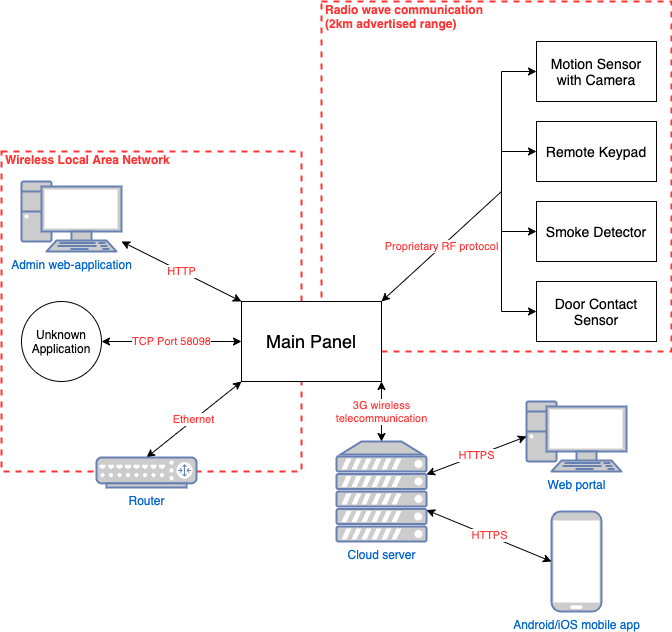
\includegraphics[width=\textwidth]{images/5-threat-model/system-overview.png}
    \caption{A data flow diagram of the system.}
    \label{fig:system-overview}
\end{figure}


\subsection{System Technologies}
Table \ref{tb:system-technologies} contains all identified technologies present in the system. There are undoubtedly additional technologies used but these are the ones identified and relevant.
\begin{table}[!p]
    \centering
    \begin{tabularx}{\textwidth}{l X}
        \hline
        \textbf{Technology}  & \textbf{Description}
        \\ \hline
        Main Panel & Linux 2.6-2.30. Hosts a web server over HTTP, using Mongoose (an embedded webserver), version unknown. Unknown application listening on TCP port 58098. Hosts DNS on TCP/UDP port 53. Has a USB and ethernet port.
        \\ \hline
        HTTP  & Protocol used by the admin web application. A clear text protocol used to communicate with the web admin panel.
        \\ \hline
        F1 RF protocol  & A proprietary \gls{RF} protocol from the hardware manufacturer, Climax Technology. Uses 868 MHz frequency. This is an undocumented protocol, meaning no technical specifications have been publicized.
        \\ \hline
        Mongoose web server  & An open-source web server, in C. Used by the main panel to host the local admin web page, version unknown. Information leaked via the HTTP \texttt{Server} header on some endpoints.
        \\ \hline
        ARM architecture  & The CPU of the main panel is an ARM (little-endian) SOC system from \textit{Grain Media}.
        \\ \hline
        3G telecommunication  & The main panel communicates with the external servers over the 3G mobile communication network.
        \\ \hline
        TCP  & The \gls{TCP} network protocol is used in communication. The main panel listens on three different TCP ports (53, 80, 58098).
        \\ \hline
    \end{tabularx}
    \caption{Technologies used in the system.}
    \label{tb:system-technologies}
\end{table}

\section{Decomposition of the system}
This section presents the results of the fourth step of the threat modeling technique. This includes all identified entry points of the system. Considering the architecture of the system, and the delimitations of this thesis, only the entry points of the main panel are presented.

As part of the decomposition of the system, all entry points of the system were identified. These are essentially all points of contact an attacker could probe. The entry points are documented in table \ref{tb:entry-points}.
\begin{table}[!ht]
    \centering
    \begin{tabularx}{\textwidth}{l X}
        \hline
        \textbf{Entry point} & \textbf{Description}
        \\ \hline
        Local web admin page  & See section \ref{ch:system:local-admin}. Provides very basic functionality but no control over the system. Has an undocumented login page via \textit{HTTP Basic Auth}. Data is transferred over HTTP on the local network.
        \\ \hline
        Unknown application  & This is a completely undocumented process, listening on TCP port 58098. Does not send any response.
        \\ \hline
        Main panel  & The physical device features an Ethernet port to connect to the local network, as well as a USB port for unknown purposes. It communicates with other devices over an 868 MHz proprietary \gls{RF} protocol.
        \\ \hline
        3G telecommunication  & The device has a SIM card and communicates over the 3G telecommunication network.
        \\ \hline
        \gls{RF} communication  & The device talks to the other peripherals over a proprietary \gls{RF} protocol, called \textit{F1}. There seems to be little to no information available to the public about this protocol, other than its operating frequency of 868 MHz.
        \\ \hline
        USB port  & The device has a USB 2.0 Type-A connector.
        \\ \hline
        Firmware  & The firmware of the system.
        \\ \hline
    \end{tabularx}
    \caption{The entry points of the main panel.}
    \label{tb:entry-points}
\end{table}

\section{Identified Threats} \label{ch:threat-model:threats}
\newcommand{\owaspref}[1]{OWASP IoT \##1}
\newcommand{\etsiref}[1]{ETSI \##1}

The following section contains all identified threats. These are categorized after the threat categories of the STRIDE model. For an explanation of the model and a description of each category see section \ref{ch:method:stride}. Note the additional category \textit{Supply chain issues}, which is a proposed extension to the model when threat modeling IoT devices \cite{guzman2017iot} (see section \ref{ch:method:threat-modeling}). The \textit{OWASP IoT top 10} \cite{owasp-iot-top10} was referenced to identify common threats that the system might be vulnerable to (see section \ref{ch:related-work:owasp}). In these threats, the OWASP IoT number is referenced as \textit{\owaspref{n}}. Similarly, the \textit{ETSI EN 303 645} standard \cite{etsi-iot-standard} for IoT manufacturers was used to identify threats (see section \ref{ch:related-work:etsi}). These are referenced below as \textit{\etsiref{n}}. Many of the threats related to the RF communication were identified through the references in section \ref{ch:related-work:hacking-iot} and \ref{ch:related-work:rf-exploit}.

\subsection{Spoofing Identity}
\begin{itemize}
    \item Spoof the remote keypad through the RF communication.
    \\ (\owaspref{7})
    \item Spoof the door contact sensor through the RF communication.
    \\ (\owaspref{7})
    \item Spoof the smoke detector through the RF communication.
    \\ (\owaspref{7})
    \item Spoof the motion detection camera through the RF communication.
    \\ (\owaspref{7})
    \item Spoof the remote keypad through the RF communication.
    \\ (\owaspref{7})
\end{itemize}

\subsection{Tampering with Data}
\begin{itemize}
    \item Replay attack on the RF communication through message blocking via jamming.
    \item Change and tamper with RF packets in transit.
    \item Send valid RF packets to the main panel, triggering events, without proper authorization.
    \\ (\owaspref{7}, \etsiref{5})
    \item Make the main panel fall back to its Ethernet connection instead of 3G telecommunication.
    \\ (\etsiref{9})
\end{itemize}

\subsection{Repudiation}
\begin{itemize}
    \item Replay attack on messages in the RF protocol between devices.
    \item Disrupt/disable logging of events.
\end{itemize}

\subsection{Information Disclosure}
\begin{itemize}
    \item Information leak in the packets of the \gls{RF} protocol.
    \\ (\etsiref{5})
    \item Weak or non-existent encryption in the \gls{RF} protocol.
    \\ (\etsiref{5})
    \item Password sniffing on the local webserver.
    \\ (\etsiref{5})
    \item Leaking the existence of the system by continuous RF traffic.
    \item Extracting firmware from the main panel.
    \\ (\owaspref{10})
\end{itemize}

\subsection{Denial of Service}
\begin{itemize}
    \item Jamming of the RF protocol.
    \\ (\etsiref{5})
    \item Stop the alarm from triggering until after you've left the premises.
    \item Spamming traffic to the local webserver.
    \\ (\owaspref{2})
    \item Crash the main panel or parts of the main panel.
    \\ (\etsiref{13})
    \item Crash the external devices through the RF communication.
    \\ (\owaspref{3}, \etsiref{13})
\end{itemize}

\subsection{Elevation of Privilege}
\begin{itemize}
    \item Insecure credentials used in the system.
    \\ (\owaspref{1}, \owaspref{9}, \etsiref{1})
    \item Password attack on the local webserver login page.
    \\ (\owaspref{1}, \owaspref{9})
    \item Send valid RF packets to the main panel without proper authorization.
    \\ (\owaspref{7})
    \item Gain an authenticated connection to the main panel through one of the network services.
    \\ (\owaspref{2}, \etsiref{6})
\end{itemize}

\subsection{Supply chain issues}
\begin{itemize}
    \item Using official applications from Climax Technology to access the system, like their mobile app Vesta Home 5 \footnotelink{https://play.google.com/store/apps/details?id=com.climax.vestasmarthome.eu}{2021-04-14}.
    \\ (\owaspref{3})
    \item Using debug applications from Climax Technology to access the system. These can be found on their website \footnotelink{https://climax.com.tw/downloads/}{2021-04-14}.
    \\ (\owaspref{3})
\end{itemize}

\chapter{Penetration testing} \label{ch:pentesting}
This chapter details all penetration tests that were performed on the system. These were derived from the threat model created in chapter \ref{ch:threat-model}. All penetration tests are described in the format outlined below. If an aspect of the test was considered simple then one or more parts have been omitted.
\begin{itemize}
    \item \textit{Introduction}. Describes the attack vector that this penetration test will explore.
    \item \textit{Background}. Details the required background knowledge to perform and evaluate this penetration test, if any.
    \item \textit{Method}. Describes in detail how the test was performed, e.g in what environment, with what tools, what commands were used, etc.
    \item \textit{Results}. Describes the findings of the penetration test.
    \item \textit{Discussion}. This section contains a discussion about the reliability, validity, and generalizability of the results.
\end{itemize}

\section{Task 1: Climax Technology's Vesta platform} \label{ch:pentesting:vesta}
Climax Technology, the manufacturer of the hardware used in this system, does not seem to be a consumer-facing business. Nonetheless, they have their own software platform to control their system, called \textit{Vesta}. In the SecuritasHome system, this platform and its components are essentially replaced by \textit{Alarm.com}. The Vesta platform features a mobile application\footnotelink{https://play.google.com/store/apps/details?id=com.climax.vestasmarthome.eu}{2021-04-20} to control the system, as well as a web portal\footnotelink{https://eu.vestasmarthome.com/Vesta/}{2021-04-20}. A potential security vulnerability is if this Vesta platform is still active and usable to control this system.

\subsection{Background}
As stated above, Climax Technology have their own platform, branded as Vesta, to control the system. A common vulnerability in IoT devices is not covering up vulnerabilities arising higher up in the supply chain (\todo source). In this system, there is a possibility that \textit{Alarm.com} has not properly deactivated the access and functionality of the Vesta platform. The idea is for the Alarm.com platform to replace it entirely.

In the app \textit{Vesta Home 5 EU}, see figure \ref{fig:vesta-home-app}, one can perform essentially all actions that the Alarm.com mobile application provides (see section \ref{ch:system:software}). On the landing page, you are greeted with simple a login page (where your Alarm.com credentials don't work). However, it also includes a button labeled \textit{First Time Registration} (see figure \ref{fig:vesta-landing-page}), where one can register a new account connected to a new system. To register a new system one only needs to enter its MAC address, see \ref{fig:vesta-registration-page}, which is available without authorization from the local admin page (see \ref{ch:system:software}). Potentially, one could then register the system in the Vesta platform to gain authorization to control the system, thus bypassing the security completely.
\begin{figure}[!ht]
    \centering
    \begin{subfigure}[t]{0.5\textwidth}
        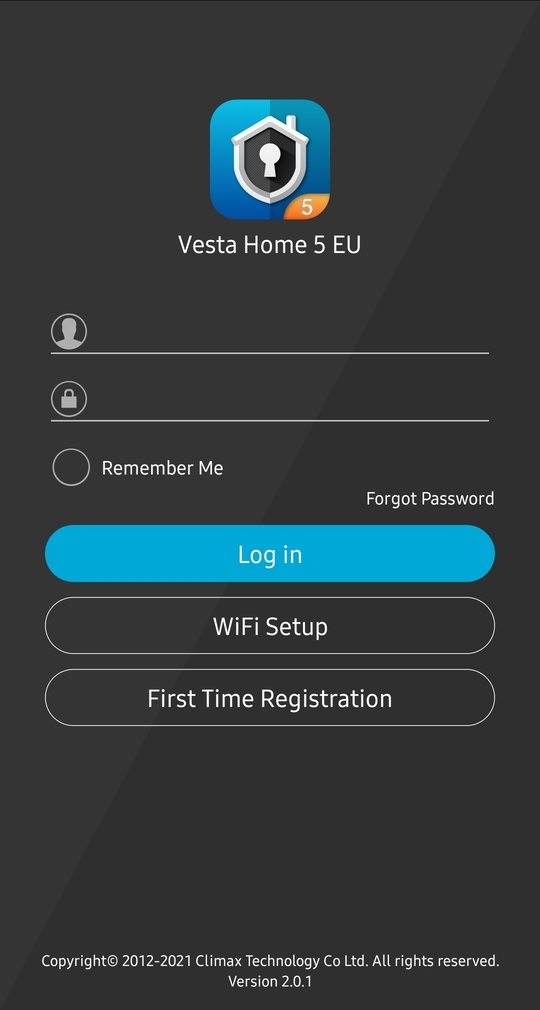
\includegraphics[height=4.8in]{images/6-pentesting/vesta-home-landing-page.jpg}
        \caption{The landing page}
        \label{fig:vesta-landing-page}
    \end{subfigure}%
    ~
    \begin{subfigure}[t]{0.5\textwidth}
        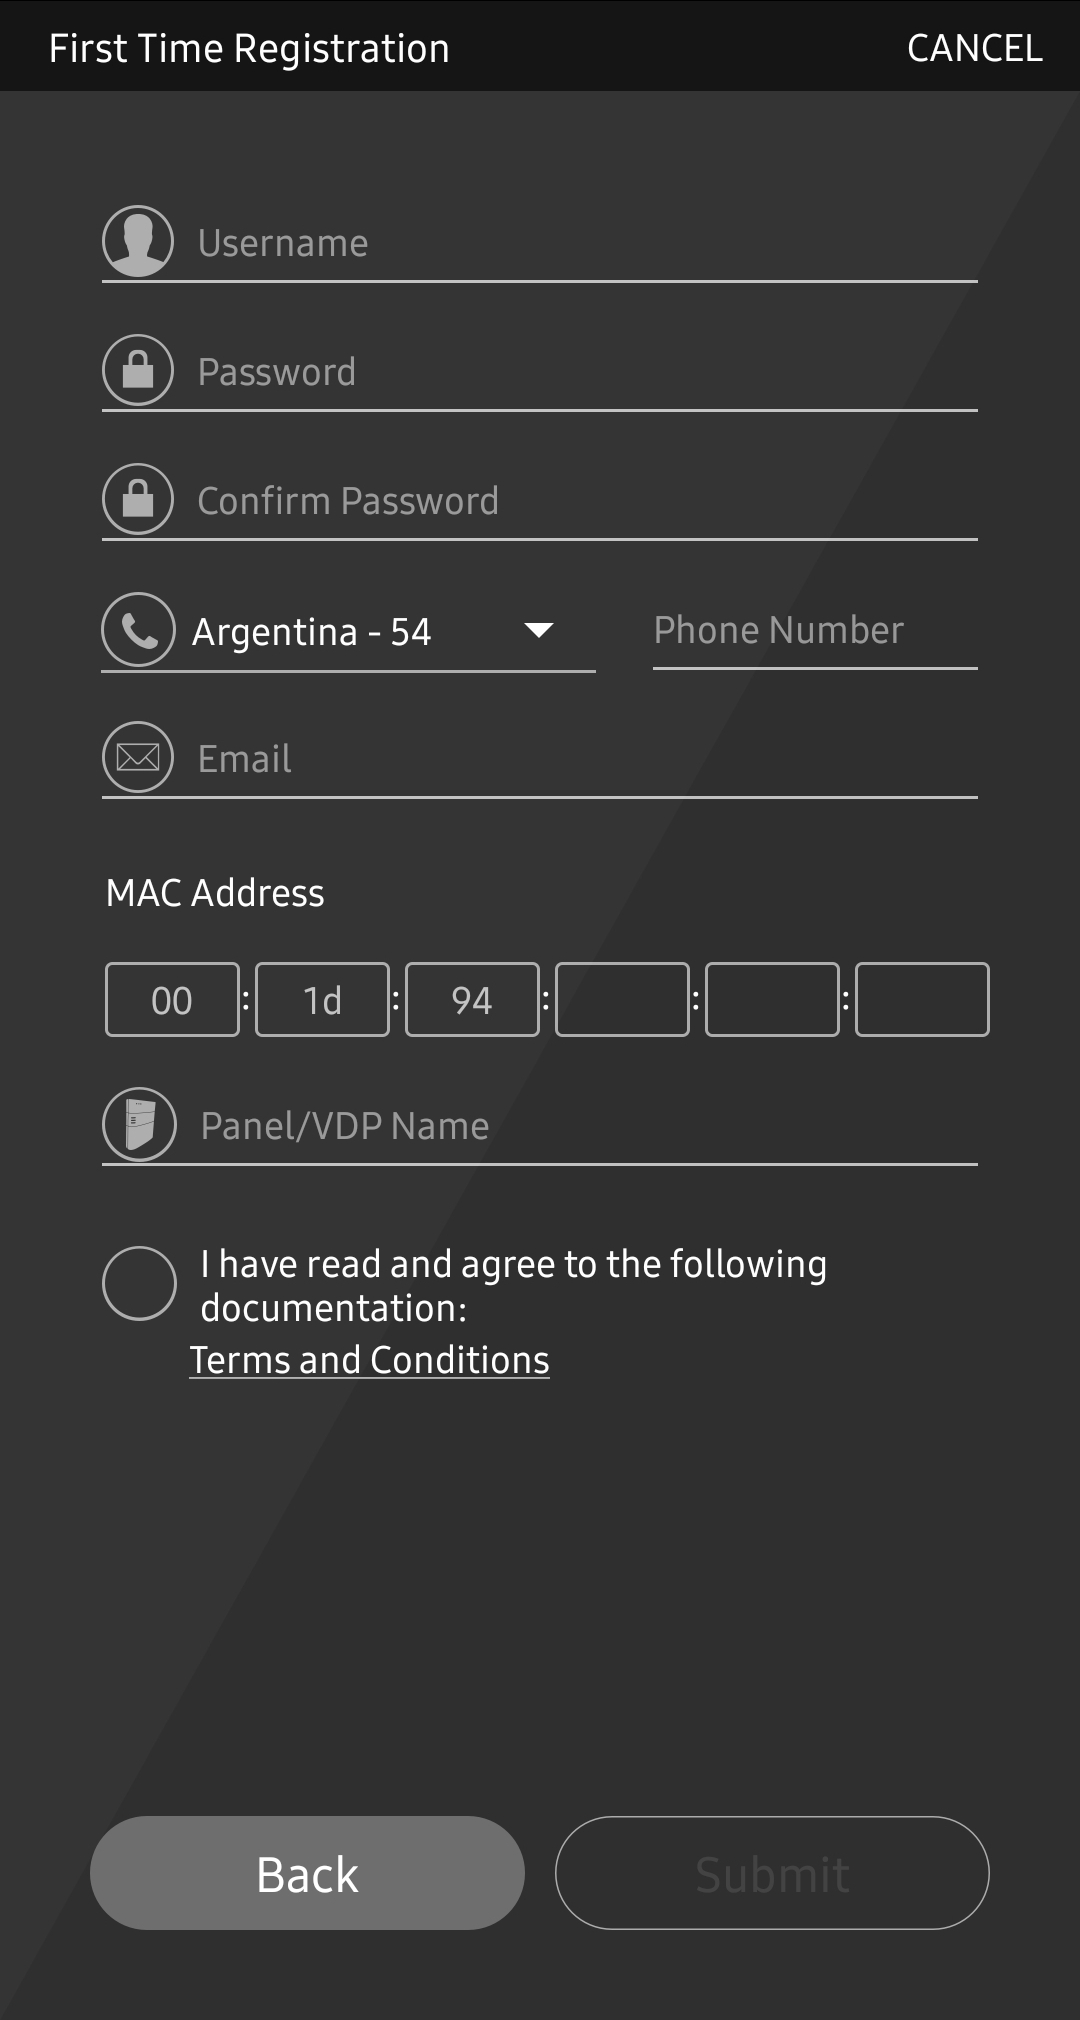
\includegraphics[height=4.8in]{images/6-pentesting/vesta-home-registration.jpg}
        \caption{The "First Time Registration" page}
        \label{fig:vesta-registration-page}
    \end{subfigure}
    \caption{The Vesta Home 5 EU mobile application.}
    \label{fig:vesta-home-app}
\end{figure}
In the Vesta web application, there is a very similar form, allowing you to register a new device using the MAC address, see figure \ref{fig:vesta-web-registration}.
\begin{figure}[!ht]
    \centering
    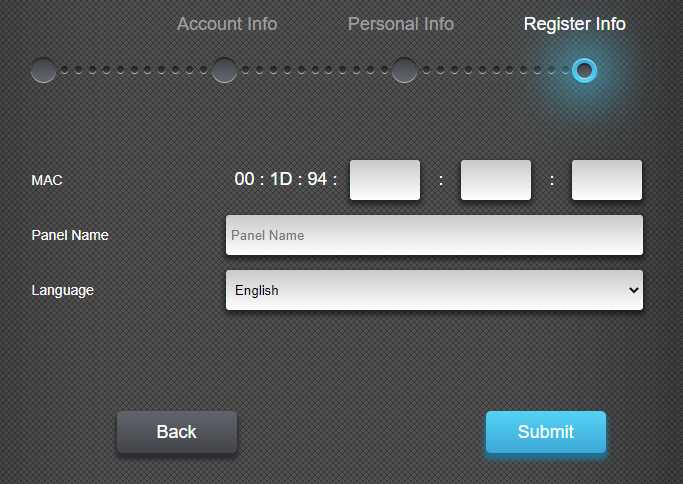
\includegraphics[width=\textwidth]{images/6-pentesting/vesta-web-registration.png}
    \caption{The Vesta web application registration.}
    \label{fig:vesta-web-registration}
\end{figure}

\subsection{Method}
The mobile application is free to download. To be able to confidently monitor the network traffic, the mobile application was installed on an android emulator for PC, and Wireshark was run on the host machine.

Both applications use HTTPS, meaning the requests are encrypted. An attempt was made to perform a \gls{MITM} attack on the mobile application to view the HTTPS traffic, using \textit{mitmproxy}\footnotelink{https://mitmproxy.org/}{2021-04-21} and the built-in proxy settings of the android emulator. However, this made the application yield an error message saying it could not reach the server. Presumably, the application uses certification pinning to protect against this type of attack. This was not explored further since the traffic can easily be viewed in the web application, using the Chrome network tab (see figure \ref{fig:vesta-web-registration-failed}), and most likely both applications access the same API.

\subsection{Results}
The penetration test was unsuccessful. Both the mobile application and the web application yielded identical results. A simple error message is shown, saying the \textit{MAC/IMEI} is incorrect, see figures \ref{fig:vesta-home-registration-failed} and \ref{fig:vesta-web-registration-failed}. In the Chrome network tab, we can see when trying to register the system through the web application that the API responds with the message "no data found!".
\begin{figure}[!ht]
    \centering
    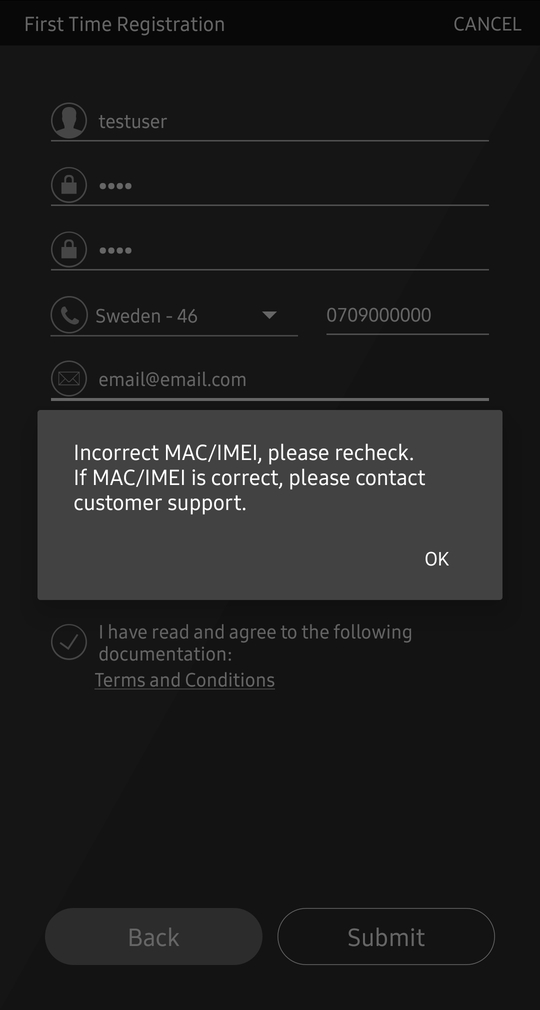
\includegraphics[width=0.4\textwidth]{images/6-pentesting/vesta-home-registration-failed.jpg}
    \caption{The results of trying to register in the mobile app.}
    \label{fig:vesta-home-registration-failed}
\end{figure}
\begin{figure}[!ht]
    \centering
    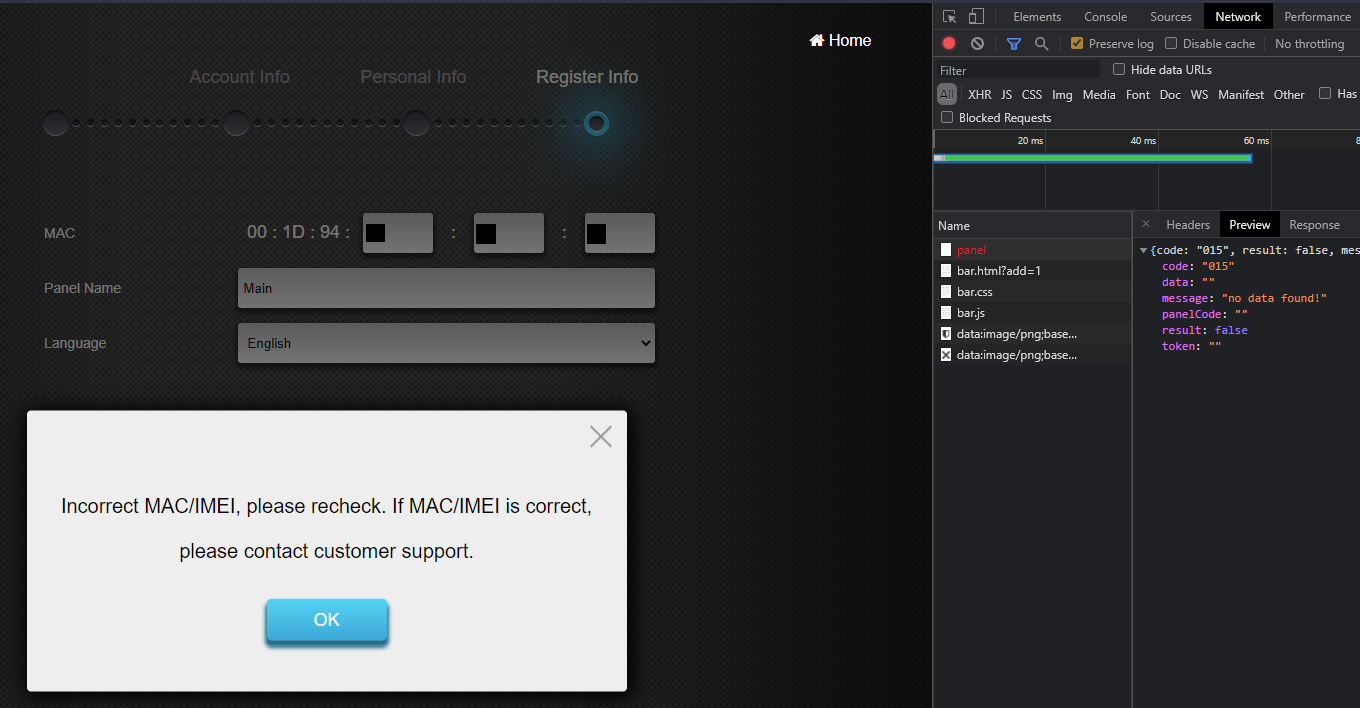
\includegraphics[width=\textwidth]{images/6-pentesting/vesta-web-registration-failed.png}
    \caption{The results of trying to register in the web app.}
    \label{fig:vesta-web-registration-failed}
\end{figure}

\subsection{Discussion}
Trying to register the hardware to the Vesta platform was unsuccessful. The given MAC address was not accepted. Presumably, Climax Technology has a database of the MAC addresses of all sold systems under the Vesta platform. While the MAC address of the system in this thesis is registered under Climax Technology, it does not seem to be registered by the Vesta platform. Another possibility is that the MAC address and IMEI number pair is not registered because \textit{Alarm.com} has used their own SIM cards and thus a different IMEI number. This is indicated by the error messages shown. Which of these scenarios is the correct one, we cannot know. Either way, we can see that the API responds with a negative result, saying that no data could be found. Therefore, this type of supply chain error seems to have been identified and correctly protected against.

\section{Task 2: Online Password Attack}
An online password attack refers to probing an active login, as opposed to an offline attack where you for example might try to crack a hash of a leaked database. This attack involves using some type of approach to test many passwords of a login form to try and find valid credentials. The local web admin page (see section \ref{ch:system}) has a login page that could potentially be brute-forced.

\subsection{Background}
A password attack, or password cracking, refers to cyber-attacks where the attacker tries to figure out valid credentials, to gain authorized access to a system. These can be categorized into two groups: offline and online password attacks. The former refers to attacks requiring no communication with the system in order to test a valid password. An example could be listening in on network traffic and seeing a password hash. One could then perform an offline password attack by trying to figure out which password produced that hash, and thus login to the system. In an online attack, the system under attack is in continuous communication with the attacker. This could be, for example, writing a script to try many different passwords on a login page of a web page. Online password attacks are generally harder to successfully perform. They are often much slower, as the communication with the system incurs a major overhead, and also poses the potential risk of getting caught in the middle of it if the administrator of the system notices the malicious traffic. Servers also often implement rate-limiting against IP addresses to combat these types of attacks and DOS attacks.

For both online and offline password attacks, there are several techniques one can use to try and guess the correct password. The simplest one is a \textit{brute-force attack}, where the attacker simply tries all possible passwords up to some length. Given $c$ possible characters in the password and a password length of $l$, there are $c^l$ possible passwords to try. This has exponential complexity in the length of the password, and will thus scale very poorly with longer passwords. Another technique is called a \textit{dictionary attack}, where the attacker uses a large list of known common passwords. Often these lists are created from actual passwords from leaked databases. For offline attacks like hash-cracking, there are additional techniques like \textit{rainbow tables}.

In the case of the system in this thesis, we have no opportunity for an offline password attack, as no information about the password such as a hash is leaked as far as the author is aware. The local admin web page does, however, feature a login page. This page uses \textit{HTTP Basic authentication} to log in to the main panel (see figure \ref{fig:local-login-page}). If this login system has not implemented any form of rate-limiting then guessing the right password might be possible, given enough time and resources.

\subsection{Method}
We know from sources like the one covered in section \ref{ch:related-work:lupus} that \textit{admin} is most likely a valid user name. This is further indicated by the official user manual from Climax Technology\footnotelink{https://fccid.io/GX9HSGWF1919/Users-Manual/Users-Manual-4873123}{2021-04-22}, which includes default login credentials with the admin user name (the credentials do not work on this system). As stated, the login form (see figure \ref{fig:local-login-page}) uses \textit{HTTP Basic authentication} to authenticate the user. A dictionary attack was performed against this login page. The well-known password list \textit{rockyou.txt}\footnotelink{https://github.com/danielmiessler/SecLists/blob/master/Passwords/Leaked-Databases/rockyou-20.txt}{2021-04-25} was used as the dictionary. A useful program to perform online password attacks is called \textit{Hydra}\footnotelink{https://github.com/vanhauser-thc/thc-hydra}{2021-04-21}, which is a command-line tool. Using the following command, Hydra was used to perform the attack:
\begin{lstlisting}[frame=tb]
    hydra -l admin       \
          -P rockyou.txt \
          192.160.1.90   \
          http-get       \
          "/action/login:A=BASIC:F=Access Denied"
\end{lstlisting}

\subsection{Results}
The test was mostly unsuccessful. A password attack against the system was successfully executed. However, Hydra only manages to perform around 23 requests per minute against the main panel, see figure \ref{fig:hydra-password-attack}. This is too slow to be able to guess enough passwords to have a meaningful probability at a correct guess.
\begin{figure}[!ht]
    \centering
    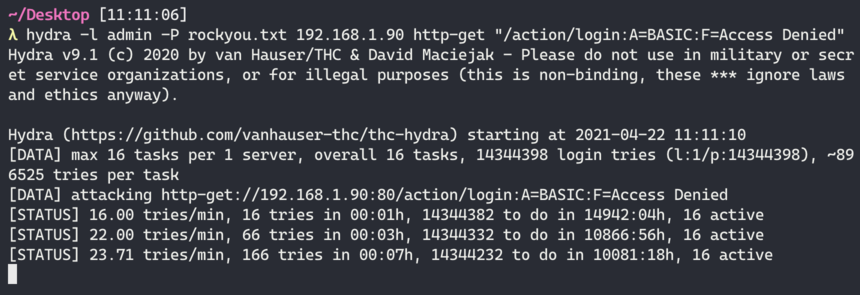
\includegraphics[width=\textwidth]{images/6-pentesting/hydra-results.png}
    \caption{The results of running a password attack.}
    \label{fig:hydra-password-attack}
\end{figure}

\subsection{Discussion}
The Hydra tool was only able to do around 23 requests per minute. Hydra is known to be very fast, so that is not the issue. One explanation for why this was so slow could be that the server rate-limits users. This is a common technique to protect against password attacks, if enough failed login attempts occur from a single IP the server would temporarily block or throttle it. However, there are signs indicating that this is not the case. For example, accessing the main web page slows down tremendously while performing the attack. Initially, it had around a \textit{16ms} response time, which increased to about \textit{17 seconds} during the attack. This was even confirmed on another computer, indicating that the main panel has not implemented any form rate-limiting per IP address. Presumably, the system is instead simply resource-bound and cannot serve requests at a faster rate. Given the hardware of the system, this is not unlikely. The CPU is most likely not that powerful, as is often the case in \gls{IOT} systems.

Due to the main panel not being able to serve more than 23 requests per minute, this type of attack is not feasible. For example, running a brute force attack, testing just all possible eight-character passwords, would take well over a hundred thousand years. A well-crafted dictionary attack could perhaps be effective, even at these slow speeds. However, there is some indication that the password might be just a random string of characters, given that the default password cited in the user manual is \texttt{cX+HsA*7F1}. If that is the case then a brute force technique is the only possibility. For these reasons, the attack was deemed unfeasible and not pursued further.

\chapter{Discussion} \label{ch:discussion}
This chapter contains a discussion about the methodology used in this report, as well as a discussion of the results found in chapter \ref{ch:pentesting}. Lastly, a mandated discussion about the sustainability and ethics of this project is presented.

\section{Methodology}
\todo

\section{Results}
\todo

\section{Sustainability and Ethics}
\todo

\chapter{Conclusions \& Future Work} \label{ch:conclusion}
This final chapter contains the conclusions drawn from the result of this thesis and a conclusion about the system's overall security. Additionally, a discussion about future work that could be done on the security of the examined system is presented.

\section{Conclusion}
Is the SecuritasHome Home Alarm System secure against cyberattacks? The answer to the research question has to be \textbf{no}. It is clear that the manufacturer has put some considerable thought into security. They use tamper sensors on all devices to protect against physical attacks, it has a battery to protect against a power outage, they use 3G telecommunication so as to not rely on the local network connection, they are able to detect jamming attacks, and they use some kind of encryption in the RF protocol (the cryptographic security of which is still in question). However, due to a glaring security flaw in the RF protocol, not protecting against replay attacks, these measures are made largely irrelevant. It goes to show how one mistake is all it takes to completely negate the security of an IT system.

Additionally, there are some bad practices found in the system, in clear violation of the ETSI EN 303 645 standard for IoT manufactures \cite{etsi-iot-standard}. One of them is leaving several network services on the system. They seemingly have no bearing on the functionality of the system and only serve to increase its attack surface, which is cause to worry.

\section{Future work} \label{ch:conclusion:related-work}
There is a lot left to examine regarding the security of the SecuritasHome smart alarm system. This project focused on the RF protocol as well as the systems network services. The results, however, showed many other promising avenues to explore which were delimited mostly due to time constraints.

Firstly, somehow acquiring the firmware of the system would open the door for a lot of interesting research. It could allow you to analyze the behavior of the \textit{58098/tcp} network service, for example, which is otherwise very difficult. One could probably the service by reverse-engineering the firmware. A possible technique to acquire the firmware would be to solder off the flash memory from the PCB and read its contents. However, that is a quite risky process that would certainly permanently break the system and possibly the flash memory in the process. The system supports over-the-air (OTA) firmware updates, however, no firmware update was sent during this entire project. Catching an OTA firmware update as it is happening is therefore quite difficult.

Additionally, one could possibly reverse engineer the encryption method used in the RF protocol by reverse-engineering the firmware. An interesting avenue is analyzing publicly available firmware from a similar system. \textit{Lupus Electronics}, as discussed in section \ref{ch:related-work:lupus}, publishes the firmware openly on their website\footnotelink{https://www.lupus-electronics.de/en/service/downloads/}{2021-06-09}. Their system is also from Climax Technology and supports F1-compatible products (the proprietary RF protocol). It is however using a different panel model. Analyzing that firmware, it is quite probable that one could reverse engineer the encryption scheme used, as well as figure out the message structure used in the protocol. However, there was not enough time to include that analysis in this thesis.

The surrounding ecosystem, including the website and mobile application, is another interesting area to explore. This was delimited early on due to both the difficulty regarding the legal aspects, and due to the interests of the author. Analyzing the android app, for example, could reveal interesting exploits. This is often quite approachable since one can decompile android APKs to something quite close to the original java source code. Analyzing the API used by both the website and mobile app is another interesting area.

% And we're done
% ( •_•)
% ( •_•)>⌐■-■
% (⌐■_■)
\noindent\rule{\textwidth}{0.4mm}


\printbibliography[title=References]

\includepdf[pages=2,pagecommand={\thispagestyle{empty}},width=\paperwidth]{kth-cover.pdf}

\divainfo{pg:lastPageofPreface}

\end{document}
